\documentclass[main.tex]{subfiles}
\setdoublesep{0.35700 em}  % 'Bond Spacing'
\setatomsep{1.78500 em}    % 'Fixed Length'
\setbondoffset{0.18265 em} % 'Margin Width'
\newcommand{\bondwidth}{0.06642 em} % 'Line Width'
\setbondstyle{line width = \bondwidth}
\newcommand\chapterlabel{acids}
\setcounter{figurenewcounter}{0}
\begin{document}




\chapter[Acids \& Bases ]{Acids \& Bases}


       \begin{marginfigure}
\begin{tikzpicture} \node (a) at (0,0) {\includegraphics[width=4cm]{chapter21/figure1}} node[rotate=90, font=\tiny] at ([yshift=.5cm,xshift=.1cm]a.south east) {\textsuperscript{\textcopyright} PngImg} ;
\end{tikzpicture}
\end{marginfigure}



   
\lettrine[lines=4]{\color{black!45}A}{cids} and bases are very important chemicals in our everyday life. Think about vinegar or Sour Patch Kids. On one hand, vinegar tastes sour as it contains acetic acid. Sour Patch Kids, on the other hand, are coated in a combination of sugar and acids. Acids help us digest food and help bacteria produce yogurt or cottage cheese. Bases on the other hand are used in drain openers, oven cleaners, or the production of soap. This chapter covers the properties of acids and bases qualitatively and quantitatively. You will learn how to identify each of these chemicals and categorize them according to their strength. Yes! acids and bases are strong, and some of them can seriously hurt you. More importantly, this chapter introduces the idea of PH, which quantifies the acidity of a solution. The PH of an acid or base depends on its strength and here we will cover how to compute the PH of solutions of strong and weak acids and bases. Balancing PH is crucial for health. Finally, we will briefly cover the idea of a buffer that helps regulate the PH of solutions and titrations used to elucidate the molarity of an unknown acid or base.


\begin{marginfigure}%LEARNING GOALS BOX
\begin{mytcbox}{GOALS}

\begin{enumerate}[label=\protect\circled{\color{white}\arabic*}]
\item Identify acids and bases and its conjugate counterparts
\item Compare the strength of two acids or bases
\item Compute the PH of solutions of weak and strong acids and bases
\item Compute titration calculations
\item Compute buffer calculations
\end{enumerate}
\end{mytcbox}
\vspace{1cm}
\begin{tcolorbox}[enhanced,colback=red!5!white,colframe=black!50!red,boxrule=1pt,
  arc=0pt,outer arc=0pt,drop heavy lifted shadow]
\faGears\ 
\docenvdef{Discussion:} {\discussionAB} \end{tcolorbox}

\end{marginfigure}%LEARNING GOALS BOX





\section{\color{blue!30!black}{The nature of acids \& Bases}}
This first section of the chapter introduces some acid-base terminology. You will learn how to identify acids and bases, and the three different models that describe acidity. More importably, you will learn what makes an acid acidic and base basic: protons and hydroxyls. 
%\begin{marginfigure}%%%%%%%% MARGIN FIGURE
%\includegraphics{chapter21/figure7}
%\caption{Citrus such as lemons or oranges are acidic. }
%\end{marginfigure}%%%%%%% MARGIN FIGURE
%  \begin{marginfigure}[0.5cm]
%\begin{tcolorbox}[enhanced,colback=red!5!white,colframe=black!50!red,boxrule=1pt,
%  arc=0pt,outer arc=0pt,drop heavy lifted shadow]
%\faGears\ 
%\docenvdef{Discussion:} List the name of three chemicals in your household that have an acid or base character and indicate its character. \end{tcolorbox}
% \end{marginfigure}
\sloppy
\begin{description}
\item[\docfilehook{How to differentiate acids and bases based on their formula}{How to differentiate acids and bases based on their formula}] In general terms, we can identify acids and bases based on its formula. Let us consider these chemicals: \ce{HF}, \ce{H2SO4} and \ce{HNO3}. All these named hydroflouric acid, sulfuric acid, and nitric acid are acidic. Hydro acids, and oxyacids will certainly be acidic. 
Acids are classified as monoprotic, diprotic and polyprotic. Monoprotic acids have only one acidic \ce{H} on its molecule (e.g. \ce{HNO3}), whereas diprotic acids have two (e.g. \ce{H2NO4}) and polyprotic acids have more than two (e.g. \ce{H3PO4}).
Hydroxides are basic and for example, \ce{NaOH} and \ce{Ca(OH)2} named sodium hydroxide and calcium hydroxide are well-known bases. At the same time, some covalent compounds such as ammonia (\ce{NH3}) are basic. However, not all covalent compounds containing hydrogen are basic and for example, \ce{CH4} is not basic at all. Finally, organic acids are acidic and organic amines tends to be basic. For example, acetic acid \ce{CH3COOH} is an acid and \ce{CH3NH2} is a base. 




%\begin{marginfigure}%%%%%%%% MARGIN FIGURE
%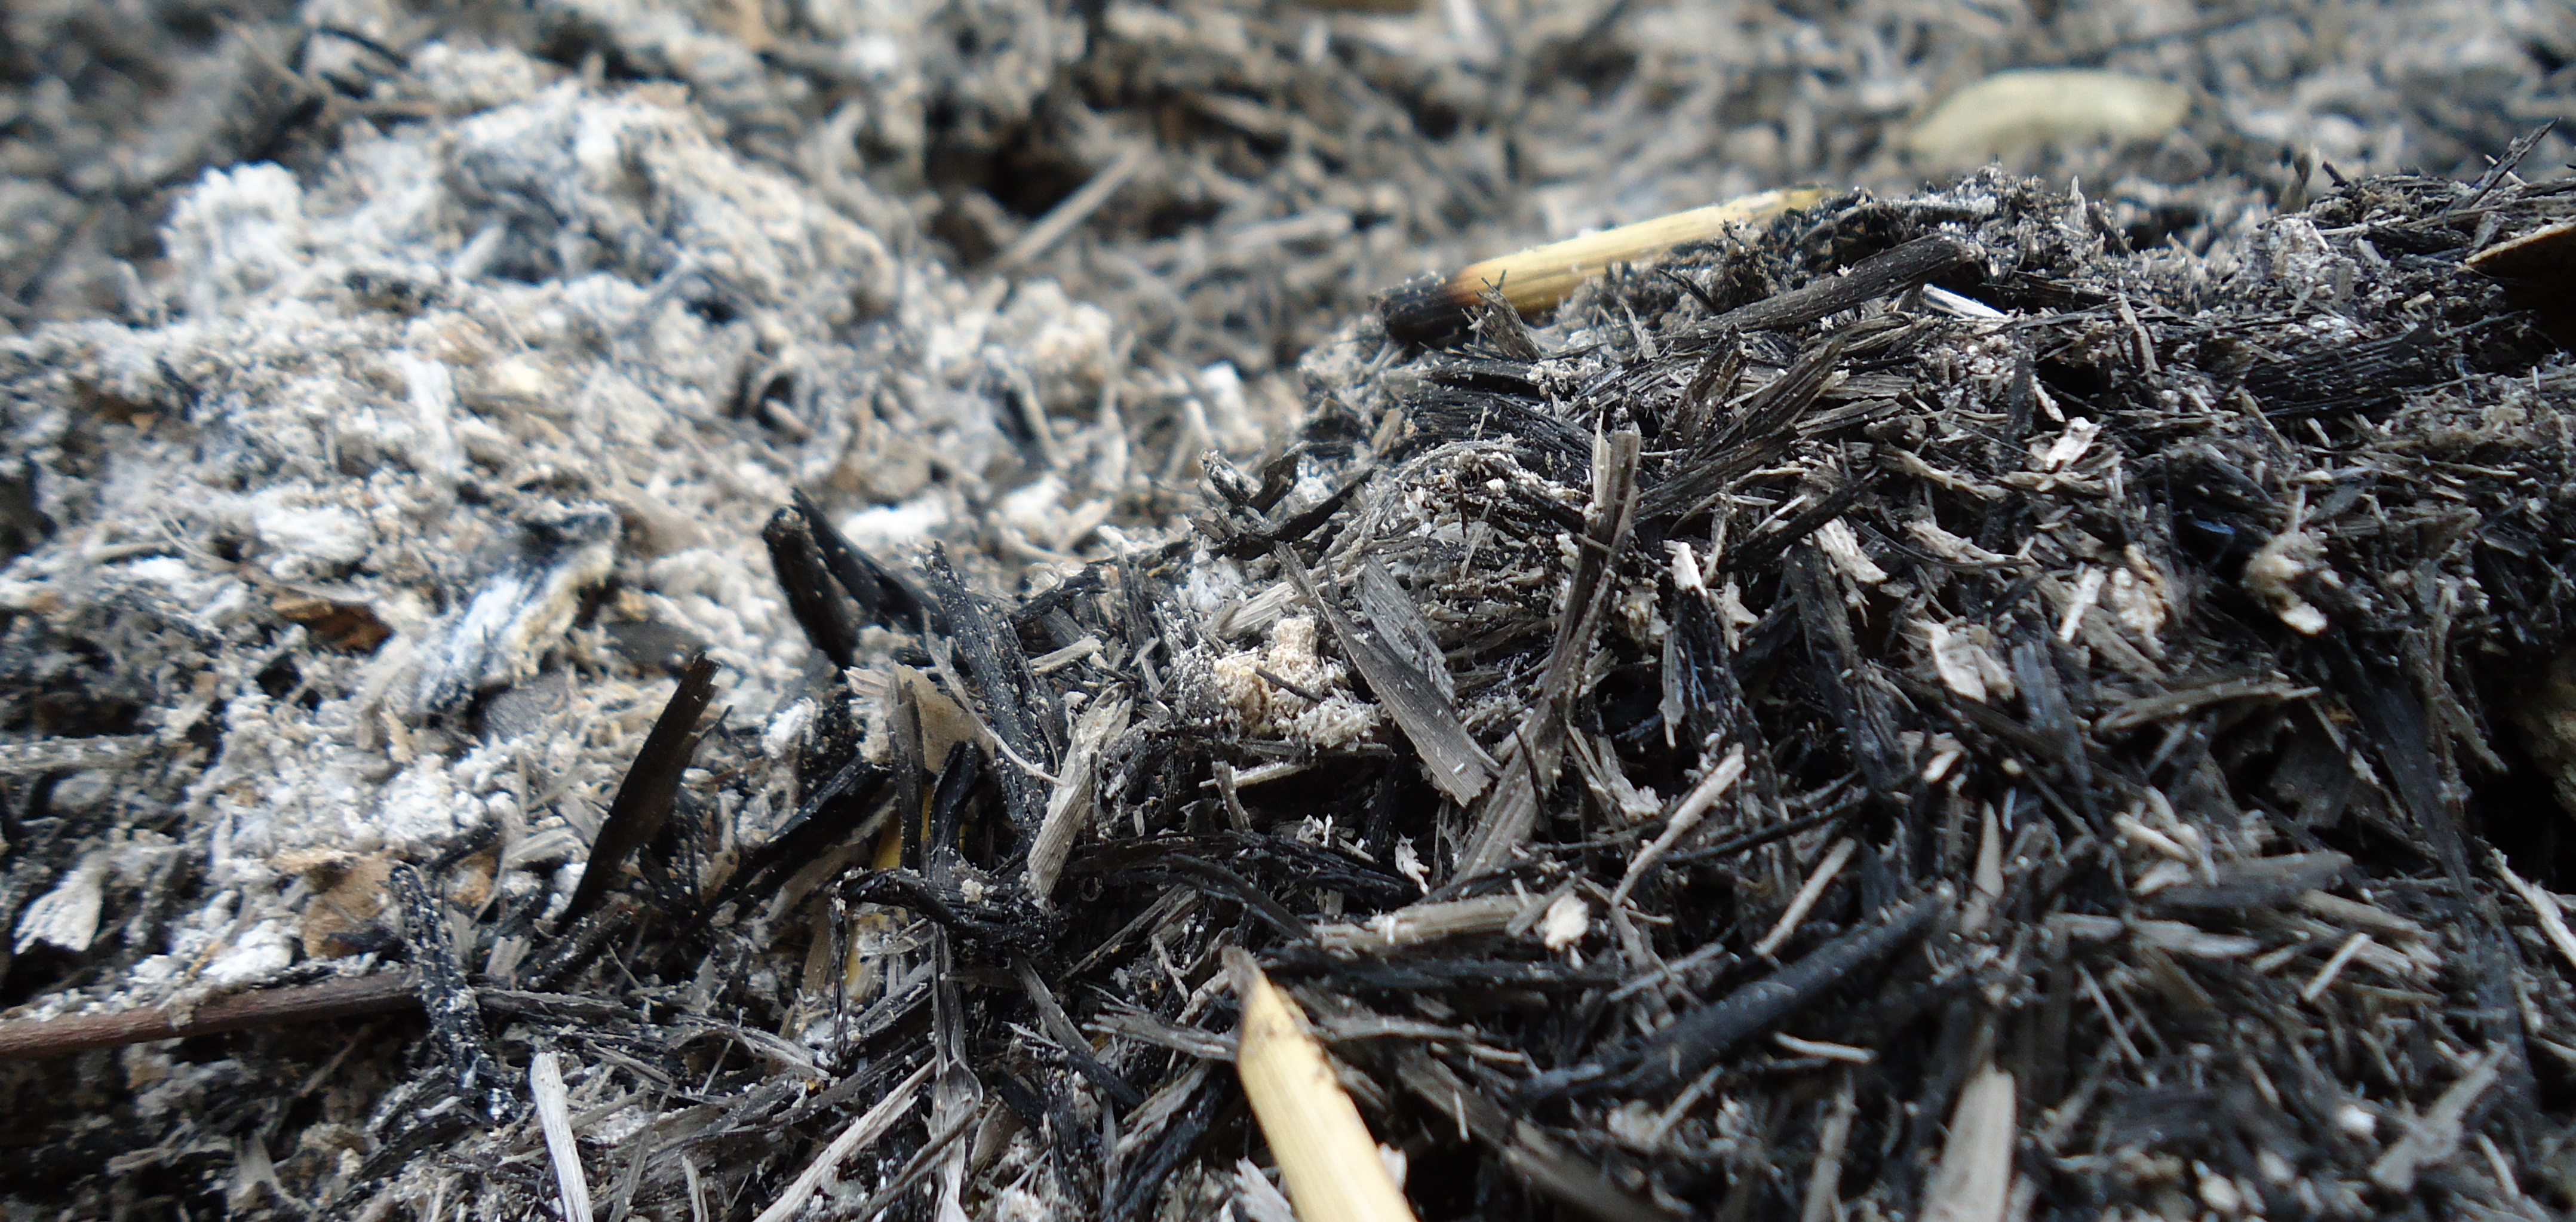
\includegraphics{chapter21/figure8}
%\caption{Ashes are basic. }
%\end{marginfigure}%%%%%%% MARGIN FIGURE

%\begin{marginfigure}%%%%%%%% MARGIN FIGURE
%\includegraphics{chapter21/figure10}
%\caption{Pickles contain vinegar that is a solution of acetic acid in water. \\ \textcolor{red}{\textbf{Q:} What is the formula for acetic acid?} }
%\end{marginfigure}%%%%%%% MARGIN FIGURE

\begin{example} %%%%%%%%%%%%%%%%%%%%%%%% EXAMPLE BOX
Identify the following chemicals as acids or bases and give their names: \ce{HCl}, \ce{NH3}, \ce{KOH}, \ce{H3PO4} and \ce{CH3COOH}.
\\
\textlcsc{ \textcolor{dgreen}{\Large \textbf{Solution}} }\\
The acids are: \ce{HCl}, \ce{H3PO4} and \ce{CH3COOH}. Their names are: hydrochloric acid, phosphoric acid and acetic acid, the later is a common name. Bases are: \ce{NH3} and \ce{KOH}. Their names are: ammonia (common name) and potassium hydroxide.
\\
\faDiamond\ \textlcsc{ \textcolor{dgreen}{\Large \textbf{Study Check}} }\\
Identify the following chemicals as acids or bases and give their names: \ce{NaOH} and \ce{H2CO3}.
\\
\flushright  {\small Answer: sodium hydroxide (base) and carbonic acid (acid). }
\end{example}%%%%%%%%%%%%%%%%%%%%%%%% EXAMPLE BOX
\item[\docfilehook{\smallpencil Acids and bases}{Acids and bases}] Acids and bases have very different properties. Acids are acidic, and this is characterized by a sour taste and often they sting to the touch. Bases are basic and that means they have a bitter--chalky--taste and they feel soapy--slippery--to the touch.
Acids are extensively used in the food and perfume industry. For example, vinegar--a liquid solution of acetic acid--is used in pickles and food preparations. On the other hand, lemon and orange juice containing citric acid is used in the preparation of effervescent salts and as a food preservative. Acids are also used in the production of batteries. Car batteries contain corrosive sulphuric acid. Bases are extensively used in manufacturing. Sodium hydroxide is used in the manufacture of soap, medicines, and even paper. Calcium hydroxide--also known as slaked lime--is used to neutralize the acid in water supplies or as an antidote for food poisoning. Calcium hydroxide is also used in the construction industry, mixed with sand and water to make mortar. Potassium hydroxide (\ce{KOH}) is also used in alkali batteries. Finally, ammonia is an extensively used cleaning product, also used to remove ink spots from clothes or grease from window-panes.\\
In the following, we will introduce the three different models used to describe acids and bases.

\item[\docfilehook{Arrhenius acid-base model}{Arrhenius acid-base model}] Arrhenius claimed that acids are acidic because when dissolved in water they produce \emph{protons}: \ce{H^+}, also called hydronium ion written as \ce{H3O^+}. Differently, bases are basic because when you solve them in water they produce \emph{hydroxyls}: \ce{OH^-}. The reaction below described the process of dissociation of hydrogen chloride to produce chloride and a proton:
\begin{center}\ce{HCl_{(g)}  <=> Cl^-_{(aq)} + H^+_{(aq)}}\hfill (an acid)\end{center}
Based on this dissociation reaction we can say hydrogen chloride also know as hydrochloric acid is an Arrhenius acid, as it produces protons. Look now the dissociation of sodium hydroxide:
\begin{center}\ce{NaOH_{(s)}   <=> Na^+_{(aq)} + OH^-_{(aq)}}\hfill (a base)\end{center}
This chemical is an Arrhenius base as it produces hydroxyls. Based on the structure of the acid is easy to tell that HCl is an Arrhenius acid as it contains hydrogen on its structure and hence it can release it giving protons. However, this model does not explain neither why chemicals unsolved in water can also be acidic nor why chemicals such as \ce{NH3} without OH on its structure can be basic.
\item[\docfilehook{Br\"{o}nsted-Lowry  acid-base model}{Br\"{o}nsted-Lowry  acid-base model}]
The second model describing acids and bases is the Br\"{o}nsted-Lowry model. This more advanced model claims acids are chemicals that give away protons (\ce{H^+}) whereas bases receive protons. Based on this mode, we can understand how acids can give away protons to water generating \ce{H3O^+} and bases such as ammonia can receive protons from water leaving \ce{OH^-} in solution:
\begin{center}\ce{NH3_{(g)} + H2O_{(l)}   <=> NH4^+_{(aq)} + OH^-_{(aq)}}\end{center}
Still, this models does not explain what structural particularity makes ammonia behave as a base and carbon dioxide (with no hydrogen on its structure) an acid.
\item[\docfilehook{Lewis acid-base model}{Lewis acid-base model}]
This is the most comprehensive acid-base model that we will cover in this chapter. A lewis acid is a chemical able to receive electron pairs, whereas bases are able to give way electron pairs. In other words, acids are electron-pair receiver and bases are electron-pair givers. In the example below you can see why ammonia acts as a base:
\begin{center}
\setatomsep{2em}
\schemestart
\chemname{\ce{H^+}}{}
\+
\chemname{\chemfig{ \lewis{4,N}( (-[:90]H)(-[:-90]H)(-[:0]H))}}{Lewis base}
\arrow{->}
\chemname{\chemfig{H-N( (-[:45,0.35,,,draw=none]\scriptstyle +)(-[:90]H)(-[:-90]H)(-[:0]H))}}{  }
\schemestop
\end{center}
Ammonia as well as other molecules contain lone pairs. These lone pairs are key in the definition of a Lewis acid-base, as acids and base receive and give away lone pairs. Lewis bases contain lone pairs and can give away electron density to an acid. 
Another example is presented below, in which the lone pairs of water make it a lewis base that can receive electron pairs from carbon dioxide, a lewis acid.
\begin{center}
\setatomsep{2.em}
\schemestart
\chemname{\chemfig{  \lewis{02,O}( (-[:-85]H)(-[:180]H))    }}{}
\+
\chemname{\chemfig{ C( (=[:90]\lewis{13,O})(=[:-90]\lewis{57,O}))}}{Lewis acid}
%\arrow{->}
%\chemname{\chemfig{  \lewis{2,O}( (-[:45,0.45,,,draw=none]\scriptstyle +)(-[:-90]H)(-[:180]H))-C( (-[:90]\lewis{024,O}(-[:45,0.45,,,draw=none]\scriptstyle {-}))(=[:-90]\lewis{57,O}))     }}{Carbonic Acid}
\arrow{->}
\chemname{\chemfig{  H^+   }}{}
\+
\chemname{\chemfig{  \lewis{2,O}( (-[:-99]H))-C( (-[:90]\lewis{024,O}(-[:45,0.45,,,draw=none]\scriptstyle {-}))(=[:-90]\lewis{57,O}))     }}{ }
\schemestop
\end{center}
In summary, the Arrhenius definition is based on what is on solution, whereas the Br\"{o}nsted-Lowry definition is based on giving and receiving protons. Finally, the Lewis definition is based on giving and receiving lone pairs. All these definitions are complementary and all Arrhenius acids are Br\"{o}nsted-Lowry as well as Lewis acids.

\begin{tcolorbox}[tab2,tabularx={X|Y|Y}]%%%% FANCY COLOR TABLE
 Model & Acid definition   &   Base definition       \\\hline\hline
Arrhenius &    \ce{H^+} producer     & \ce{OH^-} producer      \\\hline
Br\"{o}nsted-Lowry &     \ce{H^+} donnor     & \ce{H^+} acceptor    \\\hline
Lewis &   electron-pair acceptor    &  electron-pair giver   
\end{tcolorbox}%%%% FANCY COLOR TABLE


\begin{example} %%%%%%%%%%%%%%%%%%%%%%%% EXAMPLE BOX
Indicate whether the following chemicals are lewis acid or lewis bases: (a) \ce{BH3} and (b) \ce{CH_3-O-CH_3}.
\\
\textlcsc{ \textcolor{dgreen}{\Large \textbf{Solution}} }\\
The lewis structure of the molecules are:
\begin{center}
\hspace{.05in}  \chemfig{B( (-[:90]H)(-[:180]H)(-[:-90]H))} \hspace{.05in}and\hspace{.05in} \chemfig{ CH_3-\lewis{26,O}-CH_3}
\end{center}
\ce{BH3} can receive a lone pair to complete the octet of Boron and hence it will be a Lewis acid. Differently, \ce{CH_3-O-CH_3} is a Lewis base as oxygen has two lone pairs that can be given away.\\
\faDiamond\ \textlcsc{ \textcolor{dgreen}{\Large \textbf{Study Check}} }\\
Indicate whether the following chemicals are lewis acid or lewis bases: (a) \ce{AlH3} and (b) \ce{OH^{-}}.
\flushright{  \small (a) acid and (b) base.}
\end{example}%%%%%%%%%%%%%%%%%%%%%%%% EXAMPLE BOX
\end{description}


\section{\color{blue!30!black}{Dissociation of acids \& bases}}
This second section will cover the acid and base dissolution in water. Water plays a key role in the acid-base character of a chemical as these chemicals ultimately react with water. When acids and bases solve in water, they dissociate producing a byproduct called the conjugate base and conjugate acid. We will describe how to set up the dissociation equilibrium and how to identify conjugate acid-base pairs. 
\sloppy\begin{description}

\item[\docfilehook{\smallpencil Conjugate acids and bases}{Conjugate acids and bases}] A conjugate acid-base pair are molecules or ions related by the loss of one \ce{H^+}. For example: hydroiodic acid \ce{HI} and iodate \ce{l^-} or water \ce{H2O} and protons \ce{H3O^-}. The product of the dissociation of an acids is a conjugate base. For example:
\begin{center}\ce{$\textcolor{red}{\underset{\text{Acid}}{\ce{HI_{(l)}}}}$  + H2O_{(l)} -> $\textcolor{red}{\underset{\text{Conjugate Base}}{\ce{I^-_{(aq)}}}}$ + H3O^+_{(aq)}}\end{center}
Similarly, bases produce a conjugate acid. In the example below, water acts as a base and a proton is the conjugate acid:

\begin{center}\ce{$\textcolor{red}{\underset{\text{ }}{\ce{HI_{(l)}}}}$  + $\textcolor{blue}{\underset{\text{Base}}{\ce{H2O_{(l)}}}}$ -> $\textcolor{red}{\underset{\text{ }}{\ce{I^-_{(aq)}}}}$ + $\textcolor{blue}{\underset{\text{Conjugate Acid}}{\ce{H3O^+_{(aq)}}}}$}\end{center}



At the same time acids react with bases as they have opposite character. Following the previous example:
\begin{center}\ce{$\textcolor{red}{\underset{\text{Acid}}{\ce{HI_{(l)}}}}$  + $\textcolor{blue}{\underset{\text{Base}}{\ce{H2O_{(l)}}}}$ -> $\textcolor{red}{\underset{\text{Conjugate Base}}{\ce{I^-_{(aq)}}}}$ + $\textcolor{blue}{\underset{\text{Conjugate Acid}}{\ce{HI_{(l)}}}}$}\end{center}


Hence, we have that an acid reactants with an base  to produce a conjugate base and a conjugate acid. We can use the diagram below to identify the acid-conjugate base pairs:
%%%% ACID AND CONJUGATE BASE
\begin{tikzpicture}
  \node (firstleft) {Acid};
  \node [right =of firstleft] (secondleft) {Base};
  \node [right =of secondleft] (firstright) {Conjugate Base};
  \node [right =of firstright] (secondright) {Conjugate Acid};
  \node at ($(firstleft)!.5!(secondleft)$) {$+$};
  \node at ($(secondleft)!.4!(firstright)$) {\ce{->}};
  \node at ($(firstright)!.5!(secondright)$) {$+$};
  \node [above =of firstleft] (startox) {};
  \node [above =of firstright] (endox) {};
  \node [below =of secondleft] (startred) {};
  \node [below =of secondright] (endred) {};
  \draw [->] (firstleft.north) -- (startox.south) -- node[above] {\ce{H^+} loss} (endox.south) -- (firstright.north);
  \draw [->] (secondleft.south) -- (startred.north) -- node[below] {\ce{H^+} gain} (endred.north) -- (secondright.south);
\end{tikzpicture}\\
%%%% ACID AND CONJUGATE BASE


\begin{example} %%%%%%%%%%%%%%%%%%%%%%%% EXAMPLE BOX
Identify the acid, the base, the conjugate acid and the conjugate base in the reaction:
\begin{center}\ce{ NH3_{(g)} + H2O_{(l)}   -> NH4^{+}_{(aq)} + OH^-_{(aq)}}\end{center}
\textlcsc{ \textcolor{dgreen}{\Large \textbf{Solution}} }\\
The trick is first identifying the acid and the base starting for the left side of the formula. In this case \ce{NH3_{(g)}} is the base and hence water is the acid. Now connect the acid and the base with the other side of the arrow, and use conjugate with the opposite term. For example: \ce{NH3} is a base and should be related with \ce{NH4^+} that is the conjugate acid. Similarly, \ce{H2O} is a acid, being related with \ce{OH^-} that is the conjugate base. In summary:
\begin{center}\ce{$\textcolor{blue}{\underset{\text{Base}}{\ce{NH3_{(g)}}}}$ + $\textcolor{red}{\underset{\text{Acid}}{\ce{H2O_{(l)}}}}$  -> $\textcolor{red}{\underset{\text{Conjugate Acid}}{\ce{NH4^+_{(aq)}}}}$ + $\textcolor{blue}{\underset{\text{Conjugate Base}}{\ce{OH^-_{(aq)}}}}$}\end{center}
\faDiamond\ \textlcsc{ \textcolor{dgreen}{\Large \textbf{Study Check}} }\\
Identify the acid, the base, the conjugate acid and the conjugate base in the reaction:
\begin{center}\ce{ CO3^{2-}_{(aq)} + H2O_{(l)}   <=> HCO3^{-}_{(aq)} + H3O^+_{(aq)}}\end{center}
\flushright{  \small Answer: \ce{$\textcolor{blue}{\underset{\text{Base}}{\ce{CO3^{2-}_{(aq)}}}}$ + $\textcolor{red}{\underset{\text{Acid}}{\ce{H2O_{(l)}}}}$  <=> $\textcolor{red}{\underset{\text{Conjugate Acid}}{\ce{HCO3^-_{(aq)}}}}$ + $\textcolor{blue}{\underset{\text{Conjugate Base}}{\ce{H3O^+_{(aq)}}}}$}
}
\end{example}%%%%%%%%%%%%%%%%%%%%%%%% EXAMPLE BOX\end{description}


\item[\docfilehook{\smallpencil Writing down acid-base equilibria}{Writing down acid-base equilibria}] 
Now let us address how to write down acid-base equilibria from scratch, starting by the dissociation of ammonia (\ce{NH3}). Dissociation reactions are the reaction of an acid or base and water:
\begin{center}\ce{H2O_{(l)} + NH3_{(g)}   <=>  }\end{center}
We have that ammonia is a base and hence water will act as an acid. Bases receive protons whereas acids give protons away. In the equilibrium, we will remove one proton from water and add it to ammonia, producing respectively an hydroxyle and an ammonium ion:
%%%% ACID AND CONJUGATE BASE
\begin{center}\begin{tikzpicture}
  \node (firstleft) {\ce{$\textcolor{red}{\underset{\text{Acid}}{\ce{H2O^ _{(l)}}}}$}};
  \node [right =of firstleft] (secondleft) {$\textcolor{blue}{\underset{\text{Base}}{\ce{NH3_{(g)}}}}$};
  \node [right =of secondleft] (firstright) {\ce{$\textcolor{red}{\underset{\text{Conjugate Base}}{\ce{OH^-_{(l)}}}}$}};
  \node [right =of firstright] (secondright) {\ce{$\textcolor{blue}{\underset{\text{Conjugate Acid}}{\ce{NH4^+_{(aq)}}}}$}};
  \node at ($(firstleft)!.5!(secondleft)$) {$+$};
  \node at ($(secondleft)!.4!(firstright)$) {\ce{<=>}};
  \node at ($(firstright)!.5!(secondright)$) {$+$};
  \node [above =of firstleft] (startox) {};
  \node [above =of firstright] (endox) {};
  \node [below =of secondleft] (startred) {};
  \node [below =of secondright] (endred) {};
  \draw [->] (firstleft.north) -- (startox.south) -- node[above] {\ce{H^+} loss} (endox.south) -- (firstright.north);
  \draw [->] (secondleft.south) -- (startred.north) -- node[below] {\ce{H^+} gain} (endred.north) -- (secondright.south);
\end{tikzpicture}\end{center}
%%%% ACID AND CONJUGATE BASE
And that will give the dissociation equilibrium of ammonia. 
\begin{center}\ce{$\textcolor{red}{\underset{\text{Acid}}{\ce{H2O_{(l)}}}}$ + $\textcolor{blue}{\underset{\text{Base}}{\ce{NH3_{(g)}}}}$  <=> $\textcolor{red}{\underset{\text{Conjugate Base}}{\ce{OH^-_{(aq)}}}}$ + $\textcolor{blue}{\underset{\text{Conjugate Base}}{\ce{NH4^+_{(l)}}}}$}\end{center}
We can now address the reaction between an acid and a base for example, between sodium hydroxide and hydroioidic acid:
\begin{center}\ce{$\textcolor{red}{\underset{\text{Acid}}{\ce{HI_{(g)}}}}$ + $\textcolor{blue}{\underset{\text{Base}}{\ce{NaOH_{(aq)}}}}$   -> NaCl_{(aq)} + H2O_{(l)}}\end{center}
In these types of acid-base reaction, we have that the acid will generate a proton and the base will generate an hydroxyle, which will both combine to produce water and a salt, sodium chloride:

%%%% ACID AND CONJUGATE BASE
\begin{center}\begin{tikzpicture}
  \node (firstleft) {\ce{$\textcolor{red}{\underset{\text{Acid}}{\ce{HI^ _{(g)}}}}$}};
  \node [right =of firstleft] (secondleft) {$\textcolor{blue}{\underset{\text{Base}}{\ce{NaOH_{(s)}}}}$};
  \node [right =of secondleft] (firstright) {\ce{$\textcolor{red}{\underset{\text{ }}{\ce{NaCl_{(s)}}}}$}};
  \node [right =of firstright] (secondright) {\ce{$\textcolor{blue}{\underset{\text{ }}{\ce{H2O_{(l)}}}}$}};
  \node at ($(firstleft)!.5!(secondleft)$) {$+$};
  \node at ($(secondleft)!.4!(firstright)$) {\ce{->}};
  \node at ($(firstright)!.5!(secondright)$) {$+$};
  \node [above =of firstleft] (startox) {};
  \node [above =of firstright] (endox) {};
    \node [above =of secondright] (endox2) {};
  \node [below =of secondleft] (startred) {};
  \node [below =of secondright] (endred) {};
  \draw [->] (firstleft.north) -- (startox.south) -- node[above] {\ce{H^+} loss} ( endox2.south) -- (secondright.north);
  \draw [->] (secondleft.south) -- (startred.north) -- node[below] {\ce{OH^-} loss} (endred.north) -- (secondright.south);
\end{tikzpicture}\end{center}
%%%% ACID AND CONJUGATE BASE
This way, dissociation and acid-base reaction function in a very similar manner.


\begin{example} %%%%%%%%%%%%%%%%%%%%%%%% EXAMPLE BOX
Write down the following dissociation or acid-base reaction involving one proton: \ce{ H2CO3_{(aq)}  + H2O_{(aq)}   ->  }\\
\textlcsc{ \textcolor{dgreen}{\Large \textbf{Solution}} }\\
As this is a dissociation reaction and carbonic acid is an acid, we will need the help of water. We will have that carbonic acid will lose one proton and water will gain that proton.
\begin{center}\ce{ H2CO3_{(aq)}  + H2O_{(aq)}    -> HCO3^-_{(aq)} +  H3O^+_{(aq)}  }\end{center}
As carbonic acid loses a proton to become hydrogencarbonate, its charge become negative. Similarly, as water gains a proton to become the hydronium ion, its charge becomes positive so that overall the charge of the reaction is balanced.
\\
\faDiamond\ \textlcsc{ \textcolor{dgreen}{\Large \textbf{Study Check}} }\\
Write down the following dissociation or acid-base reaction involving one proton: \ce{HCl_{(g)}   +  NH3_{(g)}     ->  }\\

\flushright{  \small Answer: \ce{ HCl_{(g)}   +  NH3_{(g)}     -> NH4Cl_{(s)}   + H2O_{(l)}}
}
\end{example}%%%%%%%%%%%%%%%%%%%%%%%% EXAMPLE BOX\end{description}
\item[\docfilehook{\smallpencil Dissociating organic acids and bases}{Dissociating organic acids and bases}] 
Organic acids and bases often times contain numerous hydrogen atoms on its molecular structure. It is critical to dissociate these molecules using the acid and basic centers and not others. For example, acetic acid \ce{CH3-COOH} contains a methyl group and an carboxylic group. When dissociation this molecule, we need to remove the proton only from the acidic group, hence its name:
\begin{center}\ce{CH3-COOH_{(l)} + H2O_{(l)}   <=> CH3-COO^-_{(aq)} + H3O^+_{(aq)} }\end{center}
Methylamine \ce{CH3-NH2}, on the other hand, is an organic base with a methyl and an amine group. Amine groups are basic per nature--they resemble ammonia--and hence when dissociation this base we need to attach an extra proton to the basic center:
\begin{center}\ce{CH3-NH2_{(l)} + H2O_{(l)}   <=> CH3-NH3^+_{(aq)} + OH^-_{(aq)} }\end{center}




\item[\docfilehook{\smallpencil Strength of acids and bases}{Strength of acids and bases}] Acids and bases are indeed electrolytes. Remember electrolytes can be weak or strong depending on the degree to what they dissociate. Strong acids are strong electrolytes that dissociate completely in water producing large quantities of protons \ce{H^+}. Strong bases are strong electrolytes that dissociate completely to produce this time large quantities of hydroxyls \ce{OH^-}. Weak acid or weak bases dissociate only partially and hence they produce less protons or hydroxyls. Examples of strong electrolytes are: \ce{HCl}, \ce{H2SO4} or \ce{HNO3}. As they dissociate completely we use a single arrow to indicate the are strong electrolytes:
\begin{center}\ce{HCl(l) ->[H2O] H^+(aq) +Cl^{-}(aq)} \hspace{1cm} \textcolor{blue}{One arrow indicates strong acids or bases}\end{center}
Weak acids or basis that only dissociate partially are represented by a double arrow as the reaction is indeed an equilibrium. Examples of weak acids or bases are: \ce{NH3} or  \ce{HF}. 
\begin{center}\ce{HF(l) <=>[H2O] H^+(aq) +F^{-}(aq)} \hspace{1cm} \textcolor{blue}{A double arrow indicates weak acids or bases}\end{center}
How do we quantify the strength of an acid or base? Weak acids dissociate partially in water. And hence, the dissociation process is in equilibrium, that means you have at the same time in the same container the whole form of the acid and the conjugate base that lost its proton. For this reason, we can employ equilibrium constant $K_a$--in this chapter they are called acidity constant equivalent to $K_c$--to characterize the degree of dissociation. The larger $K_a$ the stronger the acid and hence the more protons will the acid produce in solution. Let's consider the case of \ce{HF}:
\begin{center}\ce{HF_{(l)}  <=>[H2O] H^+_{(aq)}  +F^{-}_{(aq)} } \hspace{1cm} $K_a=\frac{\big[ \ce{H^+} \big] \cdot \big[ \ce{F^-} \big]} {\big[ \ce{HF} \big] }$\end{center}
In a very similar way, bases also have what we call base dissociation constants: $K_b$. The bigger this value the stronger the base and the more hydroxyls will be produced. For the case of ammonia:
\begin{center}\ce{NH3_{(aq)} + H2O_{(l)} <=>NH4^+_{(aq)}  +OH^{-}_{(aq)} } \hspace{1cm} $K_b=\frac{\big[ \ce{NH4^+} \big] \cdot \big[ \ce{OH^-} \big]} {\big[ \ce{NH3} \big] }$\end{center}
remember liquid water can not be part of an equilibrium constant. As acids can also act as bases, there is relationship between the constant of acidity and the constant of basicity of an acid or base given by:
\begin{equation}
\boxed{ K_a\cdot K_b= 1.0\cdot 10^{-14}  }\label{\chapterlabel:equation1}
\end{equation}
For example, if the constant of acidity of a given acid is $1.5\times 10^{-5}$, the basicity constant of the same specie would be $6.6\times 10^{-10}$.

In Table \ref{tab:{\chapterlabel}1} you can find a list of some acidity and basicity constants. In general, there are some simple rules that predict the the acid-base character of an acid-conjugate base pair. Strong acids in general produce weak conjugate bases. For example, \ce{HCl} is a strong acid and its conjugate base (\ce{Cl^-}) is a weak base. Differently, \ce{HF} is a weak acid and its conjugate base (\ce{F^-}) is a moderately strong base.




   \hspace{-5cm}\begin{minipage}[b]{1.3\linewidth}

\begin{center}
        \begin{adjustbox}{center, width=\columnwidth+20pt}  % can also use \linewidth or sth. else

\refstepcounter{table} \label{tab:{\chapterlabel}1}
%\begin{table}[ht]
\fontfamily{ppl}\selectfont
\begin{tabular}{lllllll}
\rowcolor{black!45}
\toprule
\multicolumn{7}{l}{\hypersetup{colorlinks,linkcolor={white}} \cellcolor{black}\color{white}\bfseries\small Table \ref{tab:{\chapterlabel}1} Acidity and basicity constants at 25$^{\circ}$C} \\
\midrule
	\rowcolor{gray!10}Name &Formula	&$K_a$ &&  Name &Formula	&$K_a$ \\ 

\midrule
\rowcolor{red!10}\tikzmark{start} 	&							&				&&				\multicolumn{3}{c}{	 }															\\
\rowcolor{red!10} Hypoiodous acid	&		\ce{HIO}				&	$3.20 \times 10^{-11}$		&&				\multicolumn{3}{c}{	$\vdots$}															\\
\rowcolor{red!10}Phenol			&		\ce{C6H5OH}			&	$1.00 \times 10^{-10}$	 	&&	Fluoroacetic acid	&		\ce{CH2FCO2H}		&	$2.60 \times 10^{-3}$		\\
\rowcolor{red!10} Hydrocyanic acid	&		\ce{HCN}				&	$6.20 \times 10^{-10}$	 	&&	Formic acid		&		\ce{CH2O2}			&	$1.80 \times 10^{-4}$		\\	
\rowcolor{red!10}Hypobromous acid	&		\ce{HBrO}				&	$2.80 \times 10^{-9}$		&&	Bromoacetic acid	&		\ce{CH2BrCO2H}		&	$1.30 \times 10^{-3}$		\\
\rowcolor{red!10}Hypochlorous acid	&		\ce{HClO}				&	$4.00 \times 10^{-8}$		&&	Chloroacetic acid	&		\ce{CH2ClCO2H}		&	$1.30 \times 10^{-3}$		\\
\rowcolor{red!10}Benzoic acid		&		\ce{C6H5CO2H}		&	$6.25 \times 10^{-5}$		&&	Dichloroacetic acid	&		\ce{CHCl2CO2H}		&	$4.50 \times 10^{-2}$		\\
\rowcolor{red!10}Hydrazoic acid		&		\ce{HN3}				&	$2.50 \times 10^{-5}$	&&	Periodic acid		&		\ce{HIO4}				&	$2.30 \times 10^{-2}$		\\
\rowcolor{red!10}Acetic acid		&		\ce{CH3COOH}			&	$1.75 \times 10^{-5}$		&&	Chlorous acid		&		\ce{HClO2	}			&	$1.10 \times 10^{-2}$		\\
\rowcolor{red!10}Iodoacetic acid		&		\ce{CH2ICO2H}		&	$6.60 \times 10^{-4}$	&&	Trichloroacetic acid	&		\ce{CCl3CO2H}			&	$2.20 \times 10^{-1}$		\\
\rowcolor{red!10}Hydrofluoric acid	&		\ce{HF}				&	$6.30 \times 10^{-4}$		&&	Trifluoroacetic acid	&		\ce{CF3CO2H}			&	$3.00 \times 10^{-1}$		\\
\rowcolor{red!10}Nitrous acid		&		\ce{HNO2}			&	$5.60 \times 10^{-4}$		&&	Iodic acid			&		\ce{HIO3}				&	$1.70 \times 10^{-1}$		\\
\rowcolor{red!10} Cyanic acid		&		\ce{HCNO}			&	$3.50 \times 10^{-4}$		&&	Chromic acid		&		\ce{HCrO4}			&	$1.80 \times 10^{-1}$		\\
\rowcolor{red!10}\multicolumn{3}{c}{	$\vdots$}					 								&&	 			&						&				\\
\rowcolor{red!10}\tikzmark{end} 	&							&				&&				\multicolumn{3}{c}{	 }															\\
\midrule
	\rowcolor{gray!10}Name &Formula	&$K_b$ &&  Name &Formula	&$K_b$ \\ 
\midrule
\rowcolor{blue!10}\tikzmark{start2} 	&							&				&&				\multicolumn{3}{c}{	 }															\\

\rowcolor{blue!10}Aniline			&	\ce{C6H5NH2}			&	$7.40 \times 10^{-10}$	&&	\multicolumn{3}{c}{	$\vdots$}		\\
\rowcolor{blue!10}Pyridine			&	\ce{C5H5N}			&	$1.70 \times 10^{-9}$	&&	n-Butylamine		&	\ce{C4H9NH2}			&	$4.00 \times 10^{-4}$	\\
\rowcolor{blue!10}Hydroxylamine		&	\ce{NH2OH}			&	$8.70 \times 10^{-9}$	&&	Ethylamine		&	\ce{C2H5NH2}			&	$4.50 \times 10^{-4}$	\\
\rowcolor{blue!10}Hydrazine			&	\ce{N2H4}				&	$1.30 \times 10^{-6}$	&&	Methylamine		&	\ce{CH3NH2}			&	$4.60 \times 10^{-4}$	\\
\rowcolor{blue!10}Ammonia			&	\ce{NH3}				&	$1.80 \times 10^{-5}$	&&	tert-Butylamine		&	\ce{(CH3)3CNH2}		&	$4.80 \times 10^{-4}$	\\
\rowcolor{blue!10}Propylamine		&	\ce{C3H7NH2}			&	$3.50 \times 10^{-4}$	&&	Dimethylamine		&	\ce{(CH3)2NH}			&	$5.40 \times 10^{-4}$	\\
\rowcolor{blue!10}\multicolumn{3}{c}{	$\vdots$}											&&				&	&		\\
\rowcolor{blue!10}\tikzmark{end2} 	&							&				&&				\multicolumn{3}{c}{	 }															\\

  \bottomrule
\end{tabular}
\begin{tikzpicture}[overlay,remember picture]
    \draw[->] let \p1=(start), \p2=(end) in [shift={(-1,0)}]($(\x1-3,\y1)+(0.8,.2)$) -- node[rotate=90, shift={(0.0,0.4)} ] {Increasing acidic strength  } ($(\x1-3,\y2)+(0.8,1)$);
        \draw[->] let \p1=(start), \p2=(end) in [shift={(15.7,1)}]($(\x1-3,\y1)+(0.8,-1)$) -- node[rotate=90, shift={(0.0,-0.4)} ] {Increasing acidic strength  } ($(\x1-3,\y2)+(0.8,0)$);
 \draw[->] let \p1=(start2), \p2=(end2) in [shift={(-1,0)}]($(\x1-3,\y1)+(0.8,.2)$) -- node[rotate=90, shift={(0.0,0.4)} ] {Increasing basicity strength  } ($(\x1-3,\y2)+(0.8,1)$);
        \draw[->] let \p1=(start2), \p2=(end2) in [shift={(15.7,1)}]($(\x1-3,\y1)+(0.8,-1)$) -- node[rotate=90, shift={(0.0,-0.4)} ] {Increasing basicity strength  } ($(\x1-3,\y2)+(0.8,0)$);
  \end{tikzpicture}
\end{adjustbox}\end{center}
\end{minipage}







\begin{example} %%%%%%%%%%%%%%%%%%%%%%%% EXAMPLE BOX
Indicate the strongest acid from:\\
\ce{ HF_{(aq)}    <=>[H2O] H^{+}_{(aq)} + F^-_{(aq)}} \hfill $K_a=7.2\cdot 10^{-4}$\\
\ce{ HNO2_{(aq)}    <=>[H2O] H^{+}_{(aq)} + NO2^-_{(aq)}} \hfill $K_a=4.5\cdot 10^{-4}$\\
\textlcsc{ \textcolor{dgreen}{\Large \textbf{Solution}} }\\
The acid dissociation constant tells how strong is the acid, hence the larger $K_a$ the stronger the acid. Comparing both values: $K_a$(\ce{HF})$=7.2\cdot 10^{-4}$ and $K_a$(\ce{HNO2})$=4.5\cdot 10^{-4}$, \ce{HF} is the stronger of both.
\\
\faDiamond\ \textlcsc{ \textcolor{dgreen}{\Large \textbf{Study Check}} }\\
Indicate the strongest of the following acids:
\begin{center}
\ce{ H2PH4^{-}_{(aq)} + H2O_{(l)}    <=> H^{+}_{(aq)} + HPH4^{2-}_{(aq)}} \hspace{1cm} $K_a=6.2\cdot 10^{-8}$\\
\ce{   H^{+}_{(aq)} + HCO3^{2-}_{(aq)}  <=> H2CO3_{(aq)} + H2O_{(l)}} \hspace{1cm} $K_b=2.3\cdot 10^{-8}$\\
\end{center}
\flushright{  \small Answer: \ce{H2CO3} is the strongest.}
\end{example}%%%%%%%%%%%%%%%%%%%%%%%% EXAMPLE BOX

Water is a weak electrolyte.
The dissociation equilibrium of water is listed below:
\begin{center}\ce{$\textcolor{red}{\underset{\text{Acid}}{\ce{H2O_{(l)}}}}$ + $\textcolor{blue}{\underset{\text{Base}}{\ce{H2O_{(l)}}}}$  <=> $\textcolor{red}{\underset{\text{Conjugate Base}}{\ce{OH^-_{(aq)}}}}$ + $\textcolor{blue}{\underset{\text{Conjugate Acid}}{\ce{H3O^+_{(aq)}}}}$}\hfill $K_w$\end{center}
We have that water, as well as many other chemicals, can acts as a base or an acid. We call these type of chemicals \emph{amphoteric} or \emph{amphiprotic}; the last two terms are synonyms, which means they have the same meaning. Other example of amphoteric chemicals are: \ce{HCO3^-} or \ce{HSO4^-}. The dissociation constant of water is called the ion-product of water $K_w$:
\begin{center}\ce{H2O_{(l)} <=>H^+_{(aq)}  +OH^{-}_{(aq)} } \hspace{1cm} $\big[ \ce{H^+} \big] \cdot \big[ \ce{OH^-} \big]=1.0\cdot 10^{-14}$\end{center}
$K_w$ is constant that only depends on the temperature of water being $1.0\cdot 10^{-14}$ at 25$^\circ$C. The ion-product of water stablished a relationship between protons and hydroxyls in solution:
\begin{equation}
\boxed{ \big[ \ce{H^+} \big] \cdot \big[ \ce{OH^-} \big]=1.0\cdot 10^{-14}    }\label{\chapterlabel:equation2}
\end{equation}
We will explore more the use of this constant in the following sections.






%\begin{marginfigure}%%%%%%%% MARGIN FIGURE
%\includegraphics{chapter21/figure9}
%\caption{Bath bombs are made of acidic and basic ingredients that combine in water to make a fizzy bath time experience. \\ \textcolor{red}{\textbf{Q:} Which acid is used in a bath bomb?}}
%\end{marginfigure}%%%%%%% MARGIN FIGURE

\item[\docfilehook{Including water in the dissociation}{Including water in the dissociation}] Let us consider an acid such as \ce{HCl}. We know acids produce protons (\ce{H^+} or \ce{H3O^+}) so we can express the acid dissociation as:
\begin{center}\ce{HCl(l) ->[H2O] H^+(aq) + Cl^-(aq)}\end{center}
We indicate water on top of the arrow in order to represent that the dissociation process happens in water. There is an alternative way to represent this process by including explicitly water:
\begin{center}\ce{HCl_{(g)} + H2O_{(l)}	-> H3O^+_{(aq)} + Cl^-_{(aq)}}\end{center}
This way we explicitly represent the role of water as a proton receiver. Ultimately, both ways are correct and for some chemicals (e.g. \ce{NH3}) it is more convenient to use the role of water whereas for others it makes no difference.
\item[\docfilehook{Acid-base properties of salts}{Acid-base properties of salts}] Let us reming that strong acids (bases) produce weak conjugate bases (acids) and weak acids (bases) produce strong conjugate bases (acids). For example, \ce{HF} is a weak acid and therefore its conjugate \ce{F^-} acid would be strong. Similarly, \ce{NaOH} is a strong base and its conjugate acid (\ce{Na^+}) is therefore weak. Now, let us think about the acid-base properties of \ce{NaF}, a salt. Remember that salt is just a common name to refer to ionic compounds, resulting from the combination of metallic and nonmetallic elements. Without doing any type of calculation we can predict that as \ce{Na^+} is a weak acid and \ce{F^-} a strong base, a \ce{NaF} solution would be basic. Similarly, we can predict that \ce{NH4Cl} would from an acidic solution, as ammonium (\ce{NH4^+}) is the conjugate acid of ammonia (a weak base) and \ce{Cl^-} is the conjugate base of a strong acid (\ce{HCl}).




%For the case of \ce{HNO3}, nitric acid, we have:
%\begin{center}\ce{HNO3(l) ->[H2O] H^+(aq) +NO3^-(aq)}\end{center}
%that means once dissolved in water, nitric acid gives a proton and forms a nitrate \ce{NO3^-} cation. Some other acids, such as \ce{H2SO4} are diprotic, as they have two protons and hence they can loose both while reaction with water:
%\begin{center}\ce{H2SO4(l) ->[H2O] 2H^+(aq) +SO4^{2-}(aq)}\end{center}
%Bases produce hydroxyls (\ce{OH^-}) and an example of a base dissociation would be:
%\begin{center}\ce{NaOH(l) ->[H2O] Na^+(aq) + OH^-(aq)}\end{center}


%\begin{marginfigure}[0cm]%%%%%%%% MARGIN FIGURE
%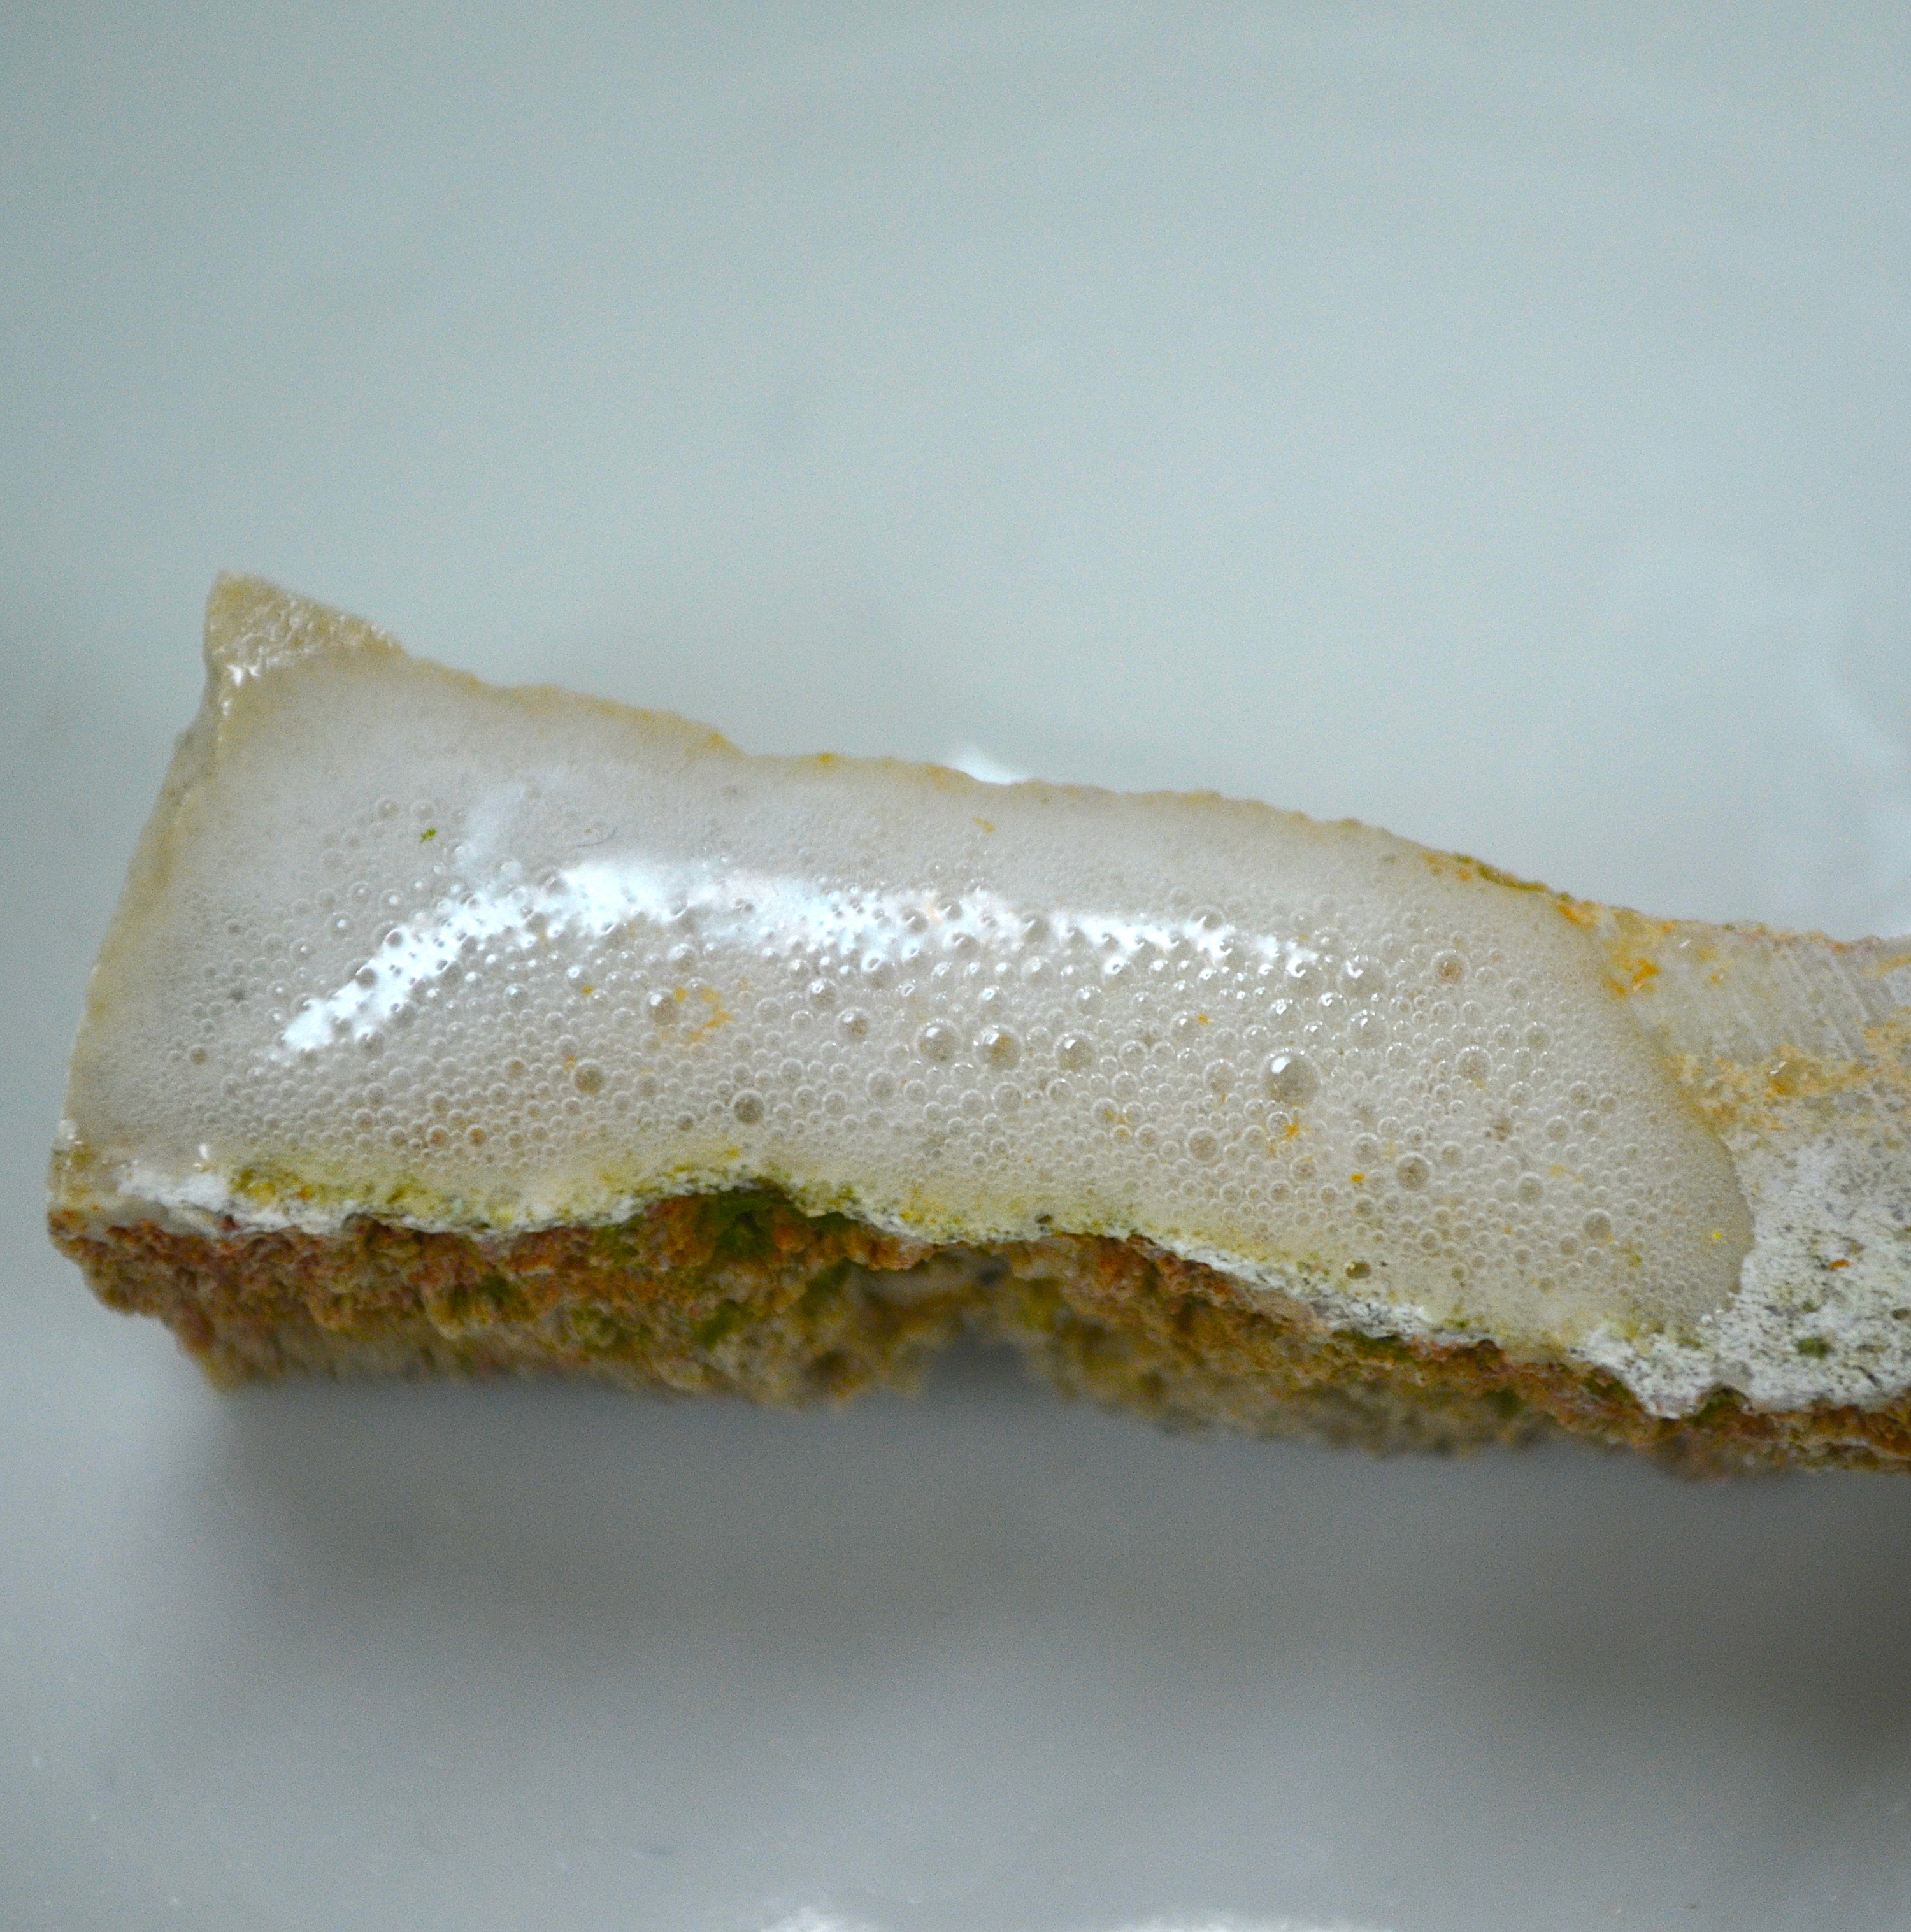
\includegraphics{chapter21/figure11}
%\caption{Limestone reactant with hydrochloric acid to give carbon dioxide bubbles. \\ \textcolor{red}{\textbf{Q:} What is the formula for limestome?}}
%\end{marginfigure}%%%%%%% MARGIN FIGURE
%\begin{marginfigure}[0cm]%%%%%%%% MARGIN FIGURE
%\includegraphics{chapter21/figure12}
%\caption{Sulfuric acid (\ce{H2SO4}) is a very strong acid.\\ \textcolor{red}{\textbf{Q:} Give the formula for two different bases conjugate of \ce{H2SO4}?}}
%\end{marginfigure}%%%%%%% MARGIN FIGURE
%\begin{marginfigure}[0cm]%%%%%%%% MARGIN FIGURE
%\includegraphics[width=0.8\columnwidth]{chapter21/figure13}
%\caption{Hydrofluoric acid is a weak acid used to dissolve glass. \\ \textcolor{red}{\textbf{Q:} Is glass an acid or a base?} }
%\end{marginfigure}%%%%%%% MARGIN FIGURE











\begin{example} %%%%%%%%%%%%%%%%%%%%%%%% EXAMPLE BOX
Write down the dissociation reaction using double arrows for the following chemicals: \ce{H3PO4_{(l)}} and \ce{NH3_{(g)}}.
\\
\textlcsc{ \textcolor{dgreen}{\Large \textbf{Solution}} }\\
Phosphoric acid is a triprotic acid with three possible protons that can be given away:
\begin{center}\ce{H3PO4_{(l)} <=>[H2O] 3H^+_{(aq)} +PO4^{3-}_{(aq)}}\end{center}
As the molecules contains protons there is no need to explicitly include water in the equilibrium. Ammonia is a base and needs is the only case in which you need to explicitly use water to help dissociate the base. This is because ammonia does not contain hydroxyls.
\begin{center}\ce{NH3_{(g)} + H2O_{(l)} <=>NH4^+_{(aq)} +OH^{-}_{(aq)}}\end{center}
\faDiamond\ \textlcsc{ \textcolor{dgreen}{\Large \textbf{Study Check}} }\\
Write down the dissociation reaction using double arrows for the following chemicals: \ce{HI_{(g)}} and \ce{HClO2_{(l)}}.
\\
\flushright{  \small Answer: \ce{HI_{(g)} <=>[H2O] H^+_{(aq)} +I^{-}_{(aq)}} and \ce{HClO2_{(l)} <=>[H2O] H^+_{(aq)} +ClO2^{-}_{(aq)}}.}
\end{example}%%%%%%%%%%%%%%%%%%%%%%%% EXAMPLE BOX\end{description}

%\begin{figure}[h] % FUL FIGURE
%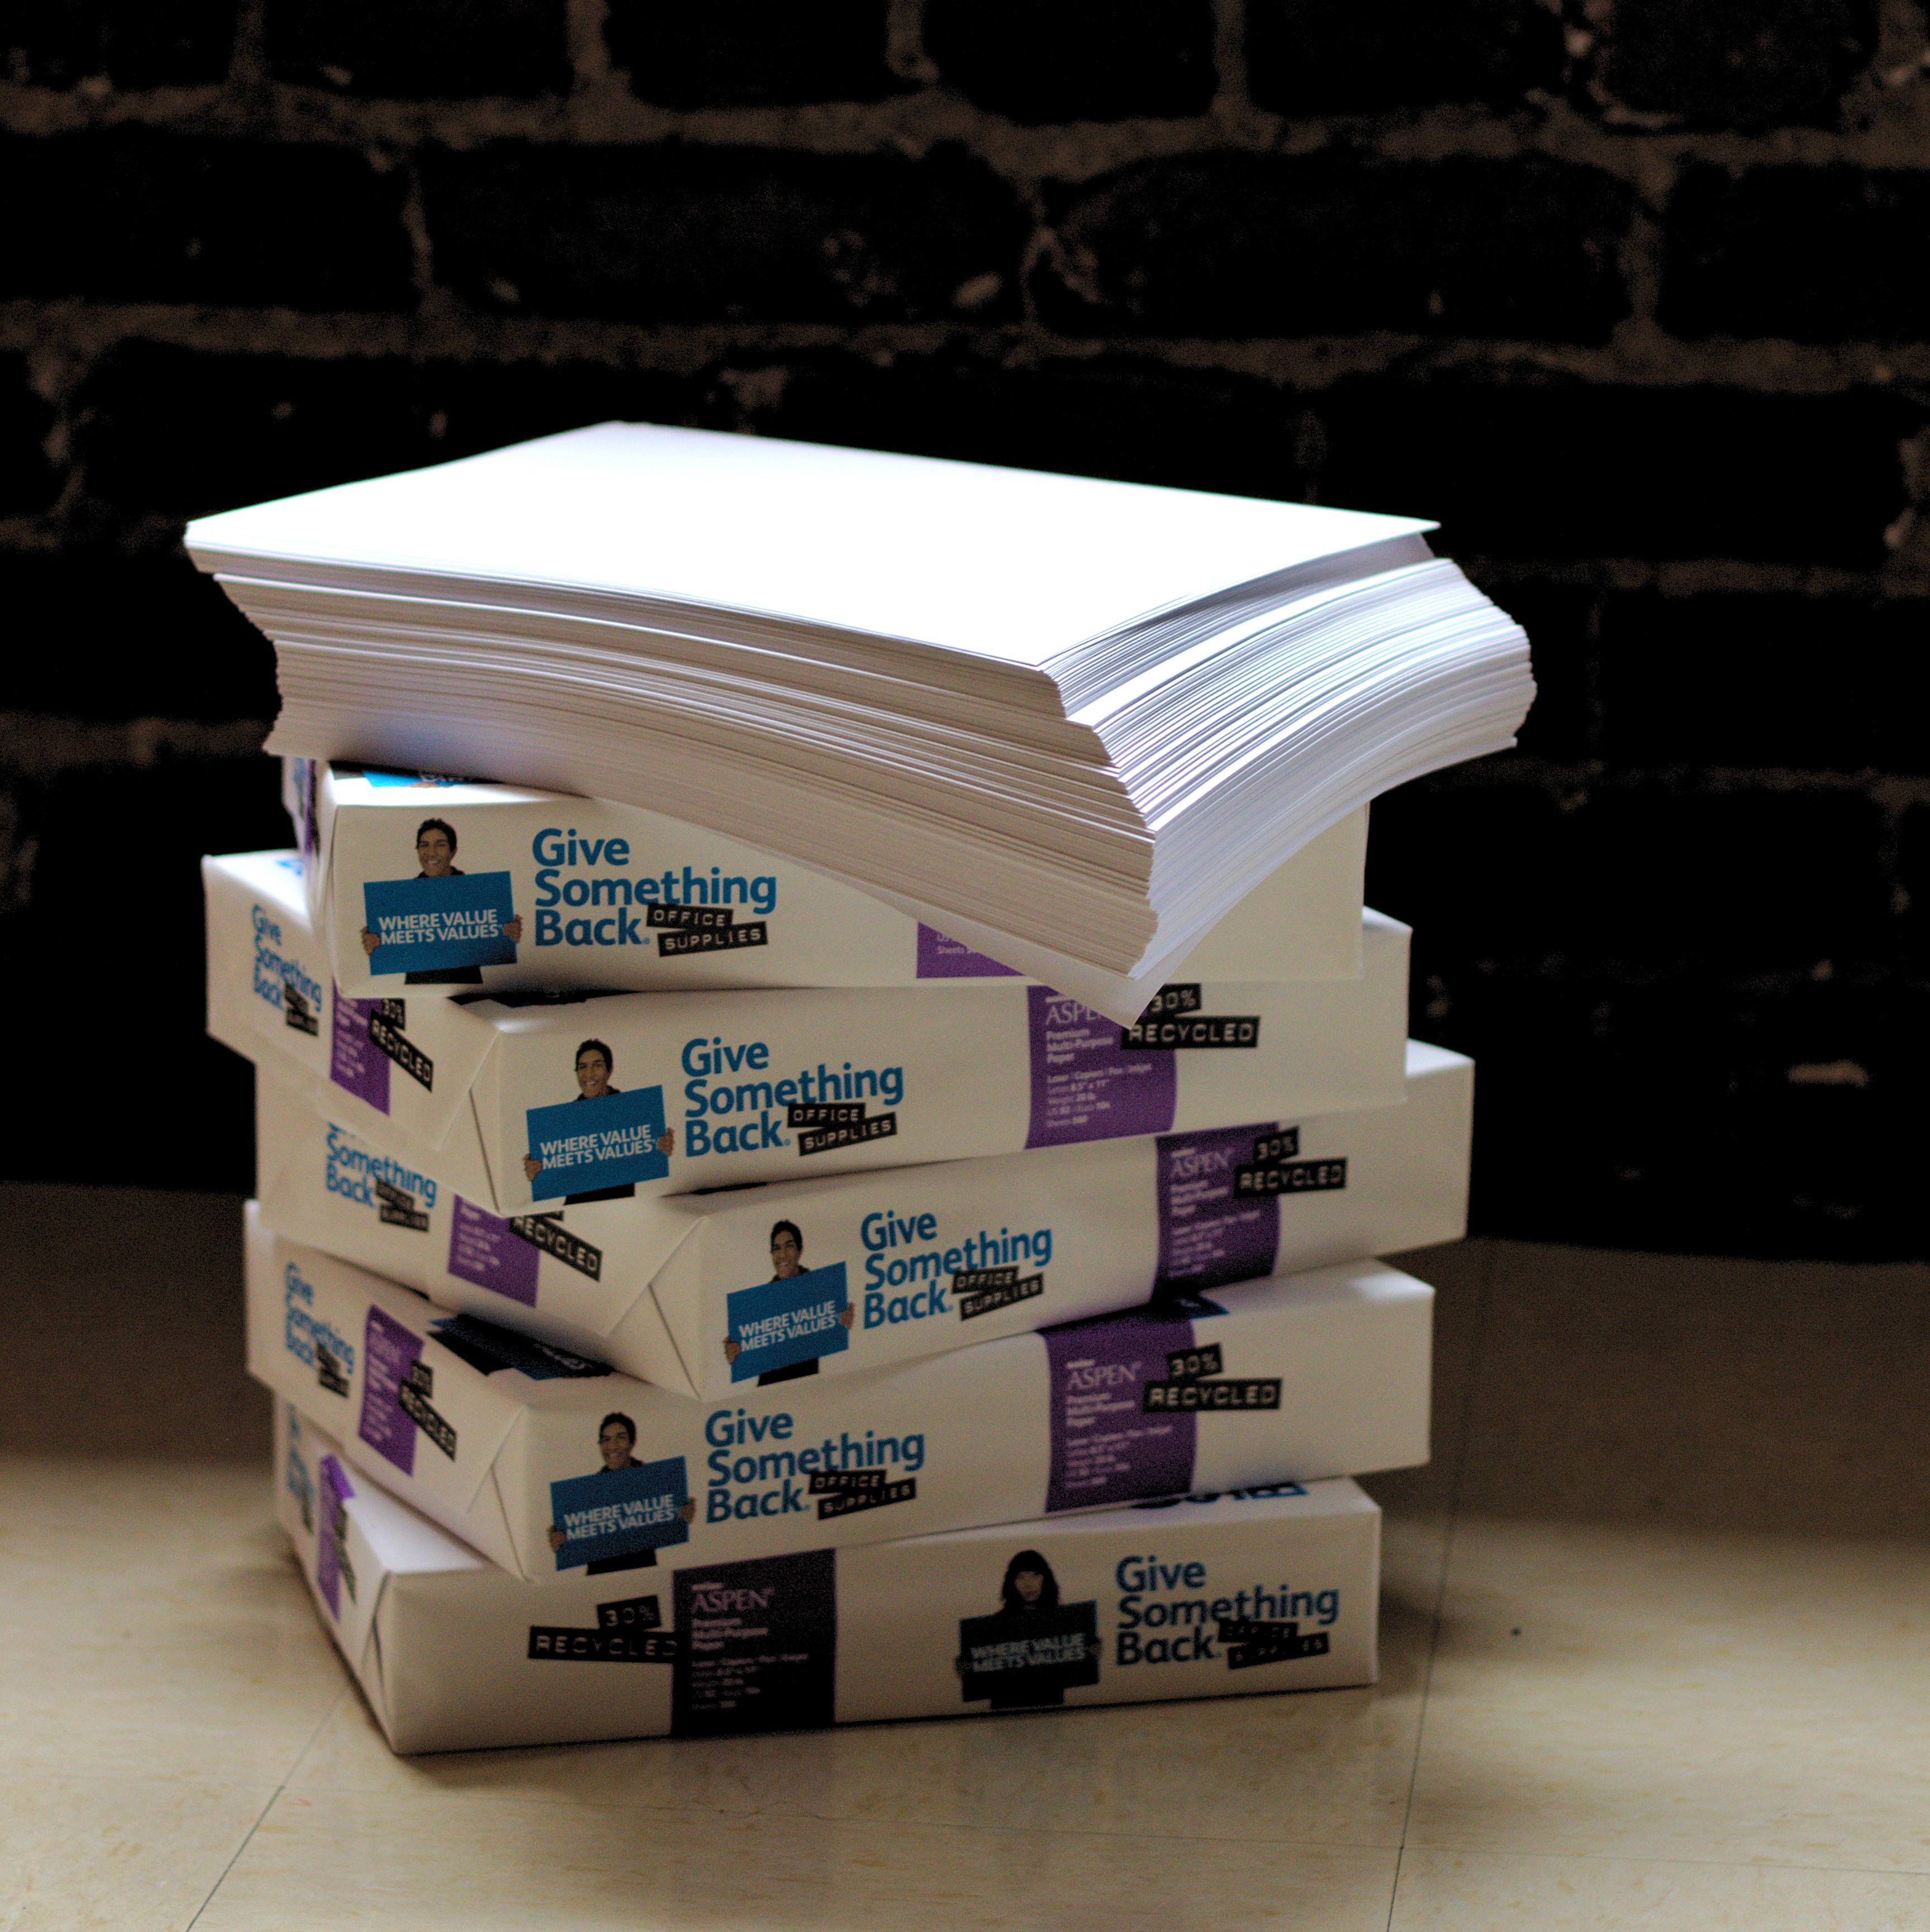
\includegraphics[width=0.8\columnwidth]{chapter21/figure14}
%\caption{Acids produce protons in water whereas bases produce hydroxyls. At the same time, acids consume hydroxyls and bases consume protons. }
%\end{figure}% FUL FIGURE




%\end{description}


%
%\section{\color{blue!30!black}{Strength of acids and bases}}
%At this point we are familiar with acids and bases. We have that acids have sour taste and produce protons in water. Differently bases feel soupy to the touch and produce hydroxyls. Both acids and bases react together giving conjugate species.  This section covers the strength of acid and bases. Some acids are weak acid whether other are stronger. The same idea can be applied to bases. We will also lear how to quantify the strength of an acid or base and compare the acidic or basic character of a chemical.
%
%\sloppy
%\begin{description}



\end{description}



\section{\color{blue!30!black}{The PH scale}}
This section describes the PH scale that simply transforms a concentration value--often times a very small number--into a simple round value. In short, the PH value tells you how much protons are there in a solution so that the larger PH the fewer protons are there in solution. It also informs about the hydroxyl concentration, as protons and hydroxyls are connected by means of the dissociation equilibrium of water.
\sloppy
\begin{description}
\item[\docfilehook{\smallpencil Protons and Hydroxyls}{Protons and Hydroxyls}] Acids and bases exist on solution with water. That means that as they produce protons or hydroxyls water receives these ions as it ionizes as well. Hence, the concentration of protons and hydroxyls in solution are not independent. Indeed, the ion-product of water relates the concentration of protons ($\big[ \ce{H^+}\big]$) and the concentration of hydroxyls ($\big[ \ce{OH^-}\big]$):
 \begin{equation*}
 \big[ \ce{H^+} \big] \cdot \big[ \ce{OH^-} \big]=1.0\times 10^{-14}
 \end{equation*}
% \resizeableyellownote{2.5}{1}{Add  Formula \textcolor{blue}{\ref{formula1}} to your flashcard.}
Water is neutral, which means that the concentration of protons ($\big[ \ce{H^+}\big]$) and the concentration of hydroxyls ($\big[ \ce{OH^-}\big]$) and both equal to $1.0\cdot 10^{-7}$M. When we dissolve an acid or a base into water, $\big[ \ce{OH^-}\big]$ and $\big[ \ce{H^+}\big]$ change drastically. When dissolving an acid, $\big[ \ce{H^+}\big]$ increases as acids produce protons, while $\big[ \ce{OH^-}\big]$ decreases. Differently, when dissolving a base,  $\big[ \ce{OH^-}\big]$ increases, as bases produce hydroxyls, while $\big[ \ce{H^+}\big]$ decreases.
 
 
\begin{example} %%%%%%%%%%%%%%%%%%%%%%%% EXAMPLE BOX
The proton concentration in an acid solution is $7.0\cdot 10^{-5}$M. Calculate $\big[ \ce{OH^-}\big]$.
\\
\textlcsc{ \textcolor{dgreen}{\Large \textbf{Solution}} }\\
We will use Equation \ref{\chapterlabel:equation2}. The value given is $\big[ \ce{H^+}\big]=7.0\cdot 10^{-5}$M and the problem ask $\big[ \ce{OH^-}\big]$. Solving for $\big[ \ce{OH^-}\big]$ we have:
\begin{equation*}
 7.0\cdot 10^{-5} \cdot \big[ \ce{OH^-} \big]=1.0\cdot 10^{-14}
 \end{equation*}
 Hence $\big[ \ce{OH^-}\big] =1.4\cdot 10^{-10}$M.
\\
\faDiamond\ \textlcsc{ \textcolor{dgreen}{\Large \textbf{Study Check}} }\\
The hydroxyl concentration in a basic solution is $2.3\cdot 10^{-6}$M. Calculate the concentration of protons.
\flushright{  \small Answer: $\big[ \ce{H^+}\big]=4.3\cdot 10^{-9}$M.}
\end{example}%%%%%%%%%%%%%%%%%%%%%%%% EXAMPLE BOX

\item[\docfilehook{\smallpencil The PH scale}{The PH scale}] The proton concentrations in aqueous solutions tend to be rather small. For example, the proton concentration in normal vinegar is $2\cdot 10^{-3}$M. As it is hard to work with these small concentrations, scientists developed the PH scale that transforms $\big[ \ce{H^+}\big]$ into a larger number. The formula for the PH is:
\begin{equation}
\boxed{PH=-log \big[ \ce{H^+} \big]  }\label{\chapterlabel:equation3}
\end{equation}

 
%\resizeableyellownote{2.5}{1}{Add  Formula \textcolor{blue}{\ref{formula2}} to your flashcard.}
The PH scale normally ranges from 0 to 14. PH values lower than 7 correspond to acidic solutions, whereas PH values larger than 7 correspond to basic solutions. Solutions with PH of 7 are neutral. 
For example, the PH for vinegar is $-log \big( 2\cdot 10^{-3}\big)$ that is 2.69. However, it exists PH values out of the scale for very concentrated solutions. Examples of PH values and common chemicals are given in the figure below.
An equivalent scale is also defined for the concentration of hydroxyls. The POH values is defined as:
\begin{equation}
\boxed{POH=-log \big[ \ce{OH^-} \big]  }\label{\chapterlabel:equation4}
\end{equation}
The POH scale also ranges from 0 to 14. POH values lower than 7 correspond to this time to basic solutions, whereas POH values larger than 7 correspond to acidic solutions. Solutions with POH of 7 are neutral. The values of PH and POH are hence related by the following equation:
\begin{equation}
\boxed{PH + POH = 14  }\label{\chapterlabel:equation5}
\end{equation}
For example, if the PH of a solution is 4 therefore the POH will be 10. Both indicators suggest that the solution would be acidic.

\begin{figure*}[h] % FUL FIGURE
\begin{tikzpicture}
 \begin{axis}[
 scale only axis, width=0pt, height=0pt, hide axis,
 tick label style={/pgf/number format/.cd, fixed},
 colorbar,colormap/jet,
 point meta min=0,
 point meta max=14,
  colorbar horizontal,
  colorbar style={
    width=0.8\textwidth,
    xtick={0,..., 14},
    },
    ] (arrow)
   { 
  };
 \end{axis}
\node[font=\Large, anchor=south west ]  at (0cm,0cm) {Acidic}; 
\node[font=\Large, anchor=south west ]  at (6.5cm,0cm) {neutral}; 
\node[font=\Large, anchor=south west ]  at (13.5cm,0cm) {Basic}; 


\draw[dashed] (2.1,-1) -- (2.1,-3);
   \node[anchor=south west,inner sep=0] (image1) at (.1cm,-3cm) {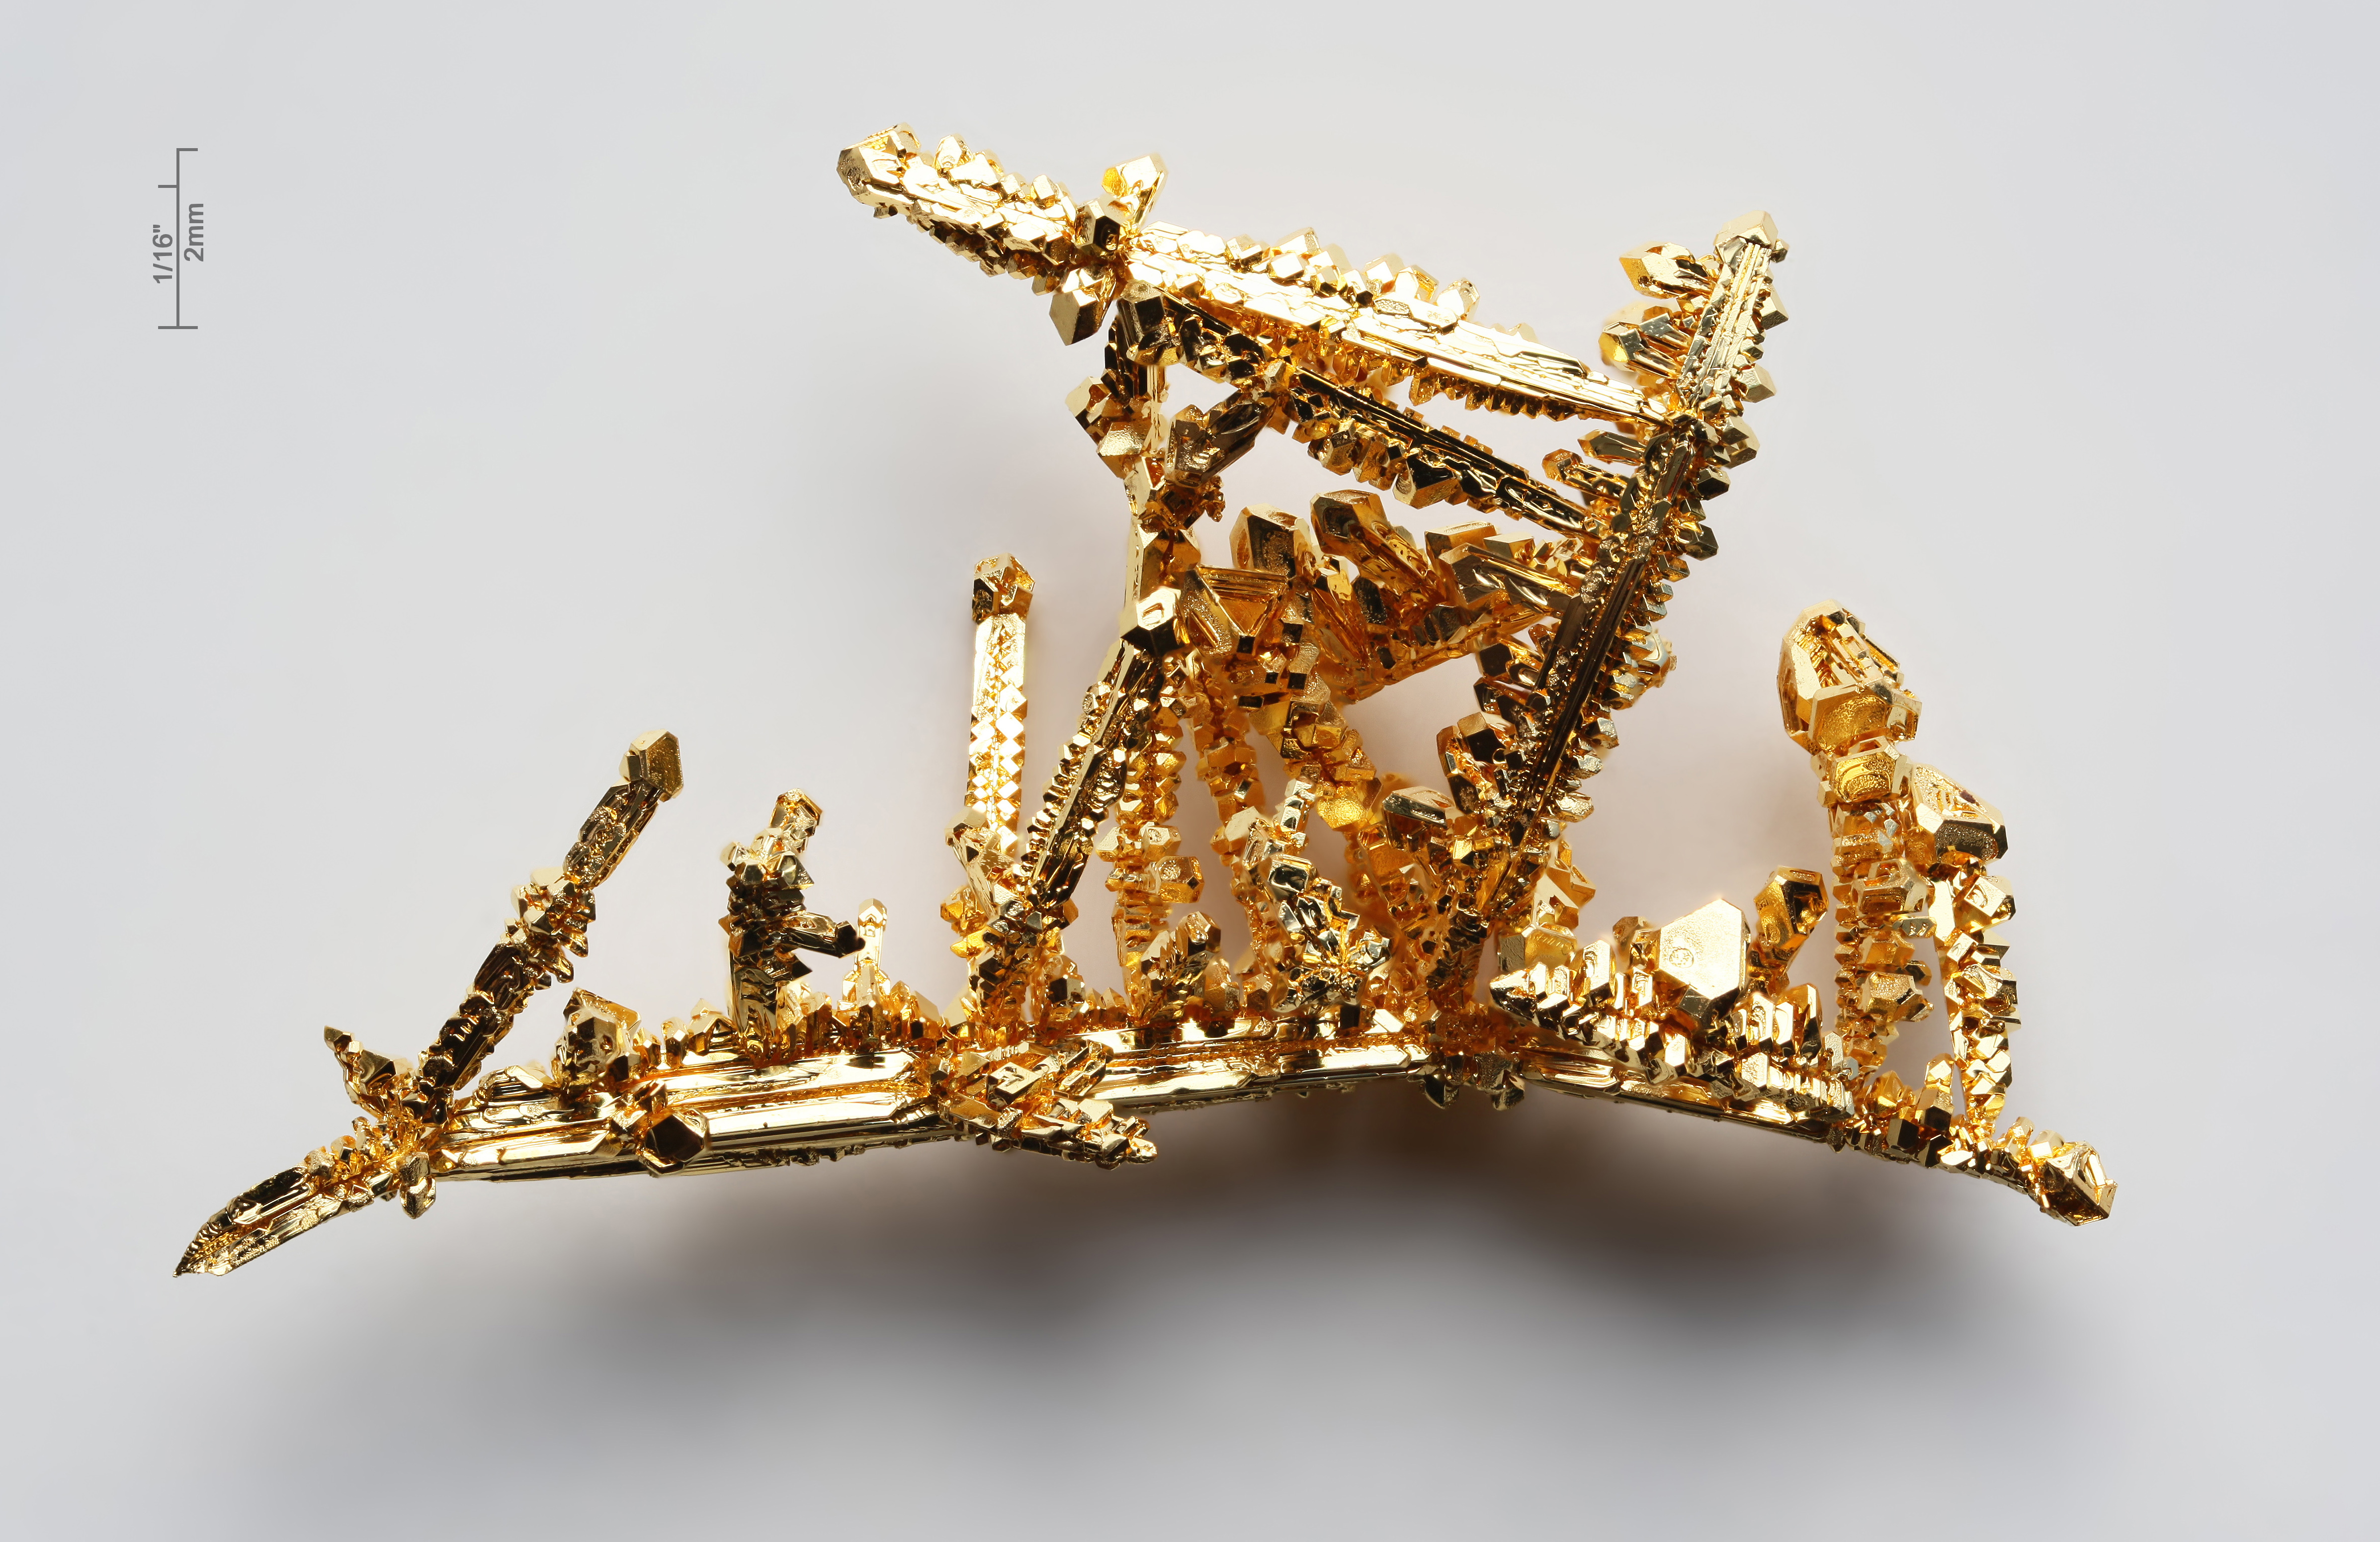
\includegraphics[width=0.1\columnwidth]{chapter21/figure6}};\node[font=\small, anchor=south west ]  at ([shift={(0.5cm,-0.5cm)}]image1.south west)  {lemon}; 
\draw[dashed] (5.25,-1.2) -- (5.25,-2);
   \node[anchor=south west,inner sep=0] (image2) at (4cm,-3cm) {\includegraphics[width=0.1\columnwidth]{chapter21/figure3}};\node[font=\small, anchor=south west ]  at ([shift={(0.5cm,-0.5cm)}]image2.south west)  {Coffee}; 
\draw[dashed] (7.3,-1) -- (7.3,-3);
   \node[anchor=south west,inner sep=0] (image2) at (7.0cm,-3cm) {\includegraphics[width=0.05\columnwidth]{chapter21/figure4}};\node[font=\small, anchor=south west ]  at ([shift={(-0.0cm,-0.5cm)}]image2.south west)  {water};
    
    \draw[dashed] (9.3,-1.2) -- (9.3,-3);
   \node[anchor=south west,inner sep=0] (image2) at (9.0cm,-3cm) {\includegraphics[width=0.05\columnwidth]{chapter21/figure5}};\node[font=\small, anchor=south west ]  at ([shift={(-0.0cm,-0.5cm)}]image2.south west)  {egg-whites};
\draw[dashed] (12.5,-1.2) -- (12.5,-3);
   \node[anchor=south west,inner sep=0] (image2) at (12.5cm,-3cm) {\includegraphics[width=0.1\columnwidth]{chapter21/figure2}};\node[font=\small, anchor=south west ]  at ([shift={(0.3cm,-0.5cm)}]image2.south west)  {chlorox};
\end{tikzpicture}
\caption{The PH scale}
\end{figure*}



\begin{example} %%%%%%%%%%%%%%%%%%%%%%%% EXAMPLE BOX
Calculate the PH for: (a) an acid solution with proton concentration of $7.0\cdot 10^{-5}$M (b) a basic solution with a hydroxyl concentration of $7.0\cdot 10^{-5}$M.
\\
\textlcsc{ \textcolor{dgreen}{\Large \textbf{Solution}} }\\
(a) We will use Equation \ref{\chapterlabel:equation3}. Given is $\big[ \ce{H^+}\big]=7.0\cdot 10^{-5}$M and the problem ask for the PH. Solving for PH we have:
\begin{equation*}
PH=-log \big(7.0\cdot 10^{-5}\big) 
 \end{equation*}
and the results is 4.15. This is an acidic PH.
(b) We will also use Equation \ref{\chapterlabel:equation3}. However, before doing that, we need to compute the concentration of protons. In order to do this we will use Equation \ref{\chapterlabel:equation2} given $\big[ \ce{OH^-} \big]=8.0\cdot 10^{-2}$M
 \begin{equation*}\big[ \ce{H^+} \big] \cdot 8.0\cdot 10^{-2}=1.0\cdot 10^{-14}\end{equation*}
We have $\big[ \ce{H^+} \big]=1.25\cdot 10^{-13}$M. Now we can compute the PH. Solving for PH we have:
\begin{equation*}
PH=-log \big(1.25\cdot 10^{-13}\big) 
 \end{equation*}
and the results is 12.90. This is a basic PH.
\\
\faDiamond\ \textlcsc{ \textcolor{dgreen}{\Large \textbf{Study Check}} }\\
Calculate the PH for: (a) an acid solution with proton concentration of $3.0\cdot 10^{-8}$M (b) a basic solution with a hydroxyl concentration of $2.0\cdot 10^{-9}$M.\\
\flushright{  \small Answer: 7.5;  5.3}
\end{example}%%%%%%%%%%%%%%%%%%%%%%%% EXAMPLE BOX







%\begin{marginfigure}[4cm]%%%%%%%% MARGIN FIGURE
%\includegraphics{chapter21/figure16}
%\caption{A PH meter is used to measure the PH of solutions. \\ \textcolor{red}{\textbf{Q:} What is the unit of PH?} }
%\end{marginfigure}%%%%%%% MARGIN FIGURE



\item[\docfilehook{\smallpencil PK of an acid or base}{PK of an acid or base}]
In the same way as we defined the PH and POH scale, we can also use the logarithmic notation to transform acidity and basicity constant into more manageable number. We define $PK_a$ of an acid as:

 \begin{equation}
\boxed{PK_a=-log \big( K_a \big) }\label{\chapterlabel:equation13}
\end{equation}
For example, as the acidity constant of acetic acid is $1.75 \times 10^{-5}$ its $PK_a$ would be 4.74. An equivalent definition exist for $PK_b$.


\item[\docfilehook{\smallpencil From PH to $\big[\ce{H^+}\big]$}{From PH to $\big[\ce{H^+}\big]$}] At this point we know that the PH quantifies the proton concentration of a solution. So given $\big[\ce{H^+}\big]$ we can calculate PH by means of the logarithm with opposite sign. But what if we know the PH and we want to calculate the corresponding proton concentration? We can do this by using the formula:
 
 \begin{equation}
\boxed{\big[\ce{H^+}\big]=\textrm{\Large 10}^{-PH} }\label{\chapterlabel:equation6}
\end{equation}


% \resizeableyellownote{2.5}{1}{Add  Formula \textcolor{blue}{\ref{formula3}} to your flashcard.}

In order to use the previous formula you need to use the power key in your calculator. For example if the PH is 3.3 and we need to calculate the proton concentration you will need to type: 10\keystroke{\large $\wedge$}\keystroke{\large $-$}3.3, and the result is $5.0\cdot 10^{-4}$M. Mind that: (a) in some calculators, sometime the power key looks like: \keystroke{\large $10^{x}$}; (b) you need to use the negative key and not the minus key. Minus is used for substations, the negative key is used for number.
An equivalent relation exist between the concentration of hydroxyls and the POH:
 \begin{equation}
\boxed{\big[\ce{OH^-}\big]=\textrm{\Large 10}^{-POH} }\label{\chapterlabel:equation7}
\end{equation}

\begin{example} %%%%%%%%%%%%%%%%%%%%%%%% EXAMPLE BOX
The PH of a solution is 4.5. Calculate the proton concentration of that solution.
\\
\textlcsc{ \textcolor{dgreen}{\Large \textbf{Solution}} }\\
We will use Equation \ref{\chapterlabel:equation6}, given PH and asking $\big[ \ce{H^+} \big]$.
\begin{equation*}
\big[\ce{H^+}\big]=\textrm{\Large 10}^{-PH}  =\textrm{\Large 10}^{-4.5} 
 \end{equation*}
and the results is $3.16\cdot 10^{-5}$M.
\\
\faDiamond\ \textlcsc{ \textcolor{dgreen}{\Large \textbf{Study Check}} }\\
The PH of a solution is 9.5. Calculate the proton concentration of that solution.
\flushright{  \small Answer: $3.16\cdot 10^{-10}$M}
\end{example}%%%%%%%%%%%%%%%%%%%%%%%% EXAMPLE BOX


The diagram below displays some of the most important equations involved in this section:


\begin{center}\begin{tikzpicture}
\node [block] (box1) at (0,0) [rectangle,draw=white,fill=red!20!white] {\textcolor{blue}{$\big[ \ce{H^+} \big]$}};
\node [block] (box2) at  (7,0) [rectangle,draw=white,fill=orange!20!white] {\textcolor{blue}{$\big[ \ce{OH^-} \big]$}};
\node [block] (box3) at  (0,5) [rectangle,draw=white,fill=yellow!20!white] {\textcolor{blue}{$\text{PH}$}};
\node [block] (box4) at  (7,5) [rectangle,draw=white,fill=green!20!white] {\textcolor{blue}{$\text{POH}$}};
%\node [block] (box5) at  (3,4) [rectangle,draw=white,fill=green!20!white] {\textcolor{blue}{Moles of H}};
\draw[thick,<->, shift={(0,0em)}] (box1.east) -- (box2.west) node[above,pos=0.5] {$ \big[ \ce{H^+} \big] \cdot \big[ \ce{OH^-} \big]=1.0\cdot 10^{-14}$} ;
\draw[thick,<->, shift={(0,0em)}] (box3.east) -- (box4.west) node[above,pos=0.5] {$ \text{PH} + \text{POH} = 14$} ;
\begin{scope}[transform canvas={xshift = -1em}]
\draw[thick,->] (box1.north)  -- (box3.south) node[above,pos=0.5, rotate=90] {$ \text{PH}=-log \big[ \ce{H^+} \big]  $} ;
\end{scope}
\begin{scope}[transform canvas={xshift = 1em}]
\draw[thick,<-] (box1.north) -- (box3.south) node[above,pos=0.5, rotate=90, yshift = -2em] {$ \big[\ce{H^+}\big]=\textrm{\Large 10}^{-\text{PH}} $} ;
\end{scope}

\begin{scope}[transform canvas={xshift = -1em}]
\draw[thick,->] (box2.north)  -- (box4.south) node[above,pos=0.5, rotate=90] {$ \text{POH}=-log \big[ \ce{OH^-} \big]  $} ;
\end{scope}
\begin{scope}[transform canvas={xshift = 1em}]
\draw[thick,<-] (box2.north) -- (box4.south) node[above,pos=0.5, rotate=90, yshift = -2em] {$ \big[\ce{OH^-}\big]=\textrm{\Large 10}^{-\text{POH}} $} ;
\end{scope}

\end{tikzpicture}\end{center}



\item[\docfilehook{\smallpencil PH of strong electrolyte solutions}{PH of strong electrolyte solutions}] Imagine we prepare a strong acid solution and we want to estimate the PH of the resulting solution. The solution PH will depend on the molarity of the resulting solution:
\begin{equation}
\boxed{PH=-log \big(n_{\ce{H}}\cdot c_a \big)  }\label{\chapterlabel:equation7}
\end{equation}
where:
\begin{where}
 \item $n_{\ce{H}}$   is the number of protons in the acid (e.g. \ce{H3PO4} has $n_{\ce{H}}$=3)
 \item $c_a$   is the molarity of the acid solution
\end{where}
We have an equivalent formula for the POH of a strong base: 
\begin{equation}
\boxed{POH=-log \big(n_{\ce{OH}}\cdot c_b \big)  }\label{\chapterlabel:equation8}
\end{equation}
where:
\begin{where}
 \item $n_{\ce{OH}}$   is the number of hydroxyls in the base  (e.g. \ce{Ca(OH)2} has $n_{\ce{OH}}$=2)
 \item $c_b$   is the molarity of the base solution
\end{where}
Mind these formulas only work for strong acids and bases, as their molarity is directly related to the concentration of protons and hydroxyls. The following example will demonstrate the use of these formulas.


\begin{example} %%%%%%%%%%%%%%%%%%%%%%%% EXAMPLE BOX
Calculate the PH of: (a) a 0.02M \ce{HNO3} solution (b) a 0.02M \ce{Ca(OH)2} solution.
\\
\textlcsc{ \textcolor{dgreen}{\Large \textbf{Solution}} }\\
(a) We will use Equation \ref{\chapterlabel:equation7} given that the molarity of the acid is 0.02M and the acid only has a single proton:
\[PH=-log \big(n_{\ce{H}}\cdot c_a \big)=-log (0.02)=1.69	\]
(b) We will use Equation \ref{\chapterlabel:equation8} given that the molarity of the base is 0.02M and it has two hydroxyls ($n_{\ce{OH}}$=2):
\[POH=-log \big(n_{\ce{OH}}\cdot c_b \big)=-log (2\cdot 0.02)=1.39\]
Now, we will convert POH in PH using Equation \ref{\chapterlabel:equation5}:
\[PH=14-POH=12.61\]
\\
\faDiamond\ \textlcsc{ \textcolor{dgreen}{\Large \textbf{Study Check}} }\\
Calculate the PH of: (a) a 0.001M \ce{H2SO4} solution (b) a 0.001M \ce{NaOH} solution.
\flushright{  \small Answer: 2.7; 11}
\end{example}%%%%%%%%%%%%%%%%%%%%%%%% EXAMPLE BOX





\item[\docfilehook{\smallpencil PH of solutions of weak acids and bases}{PH of solutions of weak acids and bases}] Imagine we prepare a weak acid solution and we want to estimate the PH of the resulting solution. The solution PH will depend on the molarity of the resulting solution. However, as weak acids and bases do not dissociate completely, the procedure and the formulas involved in the PH calculations differ from those of strong electrolytes, explained previously. In particular, for weak electrolytes, the calculation involves a quadratic equation. These equations can be solved either with the help of a graphic calculator or by means of a \faInternetExplorer \href{https://www.mathsisfun.com/quadratic-equation-solver.html}{\emph{ quadratic equation solver link}} that can be found in the internet. The resolution of quadratic formulas will lead to two different roots, a positive and a negative root. Only the positive root would make chemical sense. As such, you can directly toss the negative root.

The quadratic formula involved in the PH calculation for a weak acid is shown below:
\begin{equation}
\boxed{ \big[ \ce{H^+} \big]^2 +K_A\cdot \big[ \ce{H^+} \big] -K_a\cdot c_a=0}\;\;\;    \text{            with  }\big[ \ce{H^+} \big]=x  \label{\chapterlabel:equation9}
\end{equation}
where:
\begin{where}
 \item $\big[ \ce{H^+} \big]=x$  is concentration of protons in equilibrium
 \item $K_a$   is acidity constant of the acid
 \item $c_a$   is the molarity of the acid solution
\end{where}
For example, the PH of a 0.1M HF solution, given that HF is a weak acid with $K_a=6.3 \times 10^{-4}$, will be given by:
\[ \big[ \ce{H^+} \big]^2 +6.3 \times 10^{-4}\cdot \big[ \ce{H^+} \big] -6.3 \times 10^{-5}=0 
\]
Solving the quadratic equation, we obtain two roots: $\big[ \ce{H^+} \big]= 0.0076$ and $\big[ \ce{H^+} \big]= -0.0082 $. Only the positive root will be valid and hence we have:
\[ \big[ \ce{H^+} \big]= 0.0076\]
The PH of the solution will be 2.11.  There is an equivalent formula involved in the calculation of the PH of a weak base: 
\begin{equation}
\boxed{ \big[ \ce{OH^-} \big]^2 +K_B\cdot \big[ \ce{OH^-} \big] -K_b\cdot c_b=0}\;\;\; \text{            with  }\big[ \ce{OH^-} \big]=x \label{\chapterlabel:equation10}
\end{equation}
where:
\begin{where}
 \item $\big[ \ce{OH^-} \big]=x$  is concentration of hydroxyls in equilibrium
  \item $K_b$   is basicity constant of the base
 \item $c_b$   is the molarity of the base solution
\end{where}
Mind that in order to calculate the PH or POH you will need to employ Equations \ref{\chapterlabel:equation3} and \ref{\chapterlabel:equation4}. For example, the PH of a 0.1M \ce{NH3} solution, given that ammonia is a weak base with $K_b=1.8 \times 10^{-5}$, will be given by:
\[ \big[ \ce{OH^-} \big]^2 +1.8 \times 10^{-5}\cdot \big[ \ce{OH^-} \big] -1.8 \times 10^{-6}=0 
\]
Solving the quadratic equation, we obtain two roots: 
$ \big[ \ce{OH^-} \big]= -0.0013$ and $\big[ \ce{OH^-} \big]= 0.0013 $. Only the positive root will have chemical meaning and hence we have:
\[ \big[ \ce{OH^-} \big]= 0.0013\]
The POH of the solution will be 2.88 and the PH will be 11.11. The following example will further demonstrate the use of these formulas.
\begin{example} %%%%%%%%%%%%%%%%%%%%%%%% EXAMPLE BOX
Calculate the PH of a 0.02M  \ce{CH2O2} (formic acid) solution. $K_a=1.8 \times 10^{-4}$
\\
\textlcsc{ \textcolor{dgreen}{\Large \textbf{Solution}} }\\
As formic acid is a weak acid, we will have to use Equation \ref{\chapterlabel:equation9} in order to calculate PH:
\[\big[ \ce{H^+} \big]^2 +K_A\cdot \big[ \ce{H^+} \big] -K_a\cdot c_a=0\]
We have that $c_a$=0.02M and that $K_a=1.8 \times 10^{-4}$. Therefore $-K_a\cdot c_a$ is $-3.6 \times 10^{-6}$. Therefore, the quadratic formula that gives the PH is:
\[\big[ \ce{H^+} \big]^2 +1.8 \times 10^{-4}\cdot \big[ \ce{H^+} \big] -3.6 \times 10^{-6}=0\]
Solving for $\big[ \ce{H^+} \big]$ and using only the positive root, we have $\big[ \ce{H^+} \big]$=$1.8\times 10^{-3}$M and PH=2.74.
\\
\faDiamond\ \textlcsc{ \textcolor{dgreen}{\Large \textbf{Study Check}} }\\
Calculate the PH of a 0.002M  aniline solution. $K_b=7.4 \times 10^{-10}$
\flushright{  \small Answer: 8.08}
\end{example}%%%%%%%%%%%%%%%%%%%%%%%% EXAMPLE BOX

\item[\docfilehook{\smallpencil PH of salt solutions}{PH of salt solutions}] As well as hydracids or hydroxides, salts can exhibit acid or base character. For example, ammonium chloride (\ce{NH4Cl}) is an acidic salt, as ammonium is the conjugate acid of a weak base, and therefore has moderately strong character. Differently, chloride is the conjugate base of a strong acid (HCl) and has a weak character. Let us calculate the PH of a 0.1-M \ce{NH4Cl} solution. As the salt is acidic, we will use Equation \ref{\chapterlabel:equation9} given that $c_a$=0.1M and $K_a=5.5\times 10^{-10}$ (mind for ammonia $K_b=1.8\times 10^{-5}$ and \ref{\chapterlabel:equation1} related $K_a$ and $K_b$):
\[ \big[ \ce{H^+} \big]^2 +5.5 \times 10^{-10}\cdot \big[ \ce{H^+} \big] -5.5 \times 10^{-11}=0 \]
Solving for $\big[ \ce{H^+} \big]$ we have that $\big[ \ce{H^+} \big]=7.4\times 10^{-6}$M and PH=5.13. As predicted, the PH of an ammonium chloride solution is acidic.

\begin{example} %%%%%%%%%%%%%%%%%%%%%%%% EXAMPLE BOX
Calculate the PH of a 0.02M  \ce{HCOONa} (sodium formate) solution. $K_a=1.8 \times 10^{-4}$
\\
\textlcsc{ \textcolor{dgreen}{\Large \textbf{Solution}} }\\
Formate is the conjugate base of an weak acid, therefore it will be moderately basic. We will use \ref{\chapterlabel:equation10} given that $K_b=5.5 \times 10^{-11}$ and $c_b$=0.02M:
\[ \big[ \ce{OH^-} \big]^2 +5.5 \times 10^{-11}\cdot \big[ \ce{OH^-} \big] -5.5 \times 10^{-12}=0 \]
Solving for $\big[ \ce{OH^-} \big]$ and using only the positive root, we have $\big[ \ce{OH^-} \big]$=$2.3\times 10^{-6}$M and POH=5.63. The final answer would be: PH=8.36.
\\
\faDiamond\ \textlcsc{ \textcolor{dgreen}{\Large \textbf{Study Check}} }\\
Calculate the PH of a 0.01M sodium acetate (\ce{CH3COONa}). $K_a=1.75 \times 10^{-5}$
\flushright{  \small Answer: 8.38}
\end{example}%%%%%%%%%%%%%%%%%%%%%%%% EXAMPLE BOX




\item[\docfilehook{\smallpencil Percent dissociation of weak acids and bases}{Percent dissociation of weak acids and bases}] Weak acids (and base) are indeed weak electrolytes, which means if we prepare a solution of a given concentration $c_a$ they will dissociate giving a proton concentration ($\big[ \ce{H^+} \big]$) less than $c_a$. We define the percent dissociation $\alpha$ of an acid (or base) as:

\begin{equation}
\boxed{ \alpha=\frac{\text{amount dissociated}}{\text{initial amount}}\times 100=\frac{\big[ \ce{H^+} \big]}{c_a}\times 100 }\label{\chapterlabel:equation11}
\end{equation}
where:
\begin{where}
 \item $\big[ \ce{H^+} \big]$  is concentration of protons in equilibrium
 \item $c_a$   is initial acid concentration
\end{where}
For example, a 0.2M HF solution has a proton concentration of 0.0076M. The percent dissociation of this acid at this concentration will be 3.8\%. The percent dissociation changes with the acid (or base) concentration and more concentrated acids have in general a larger proton concentration than diluted acids. However, the percent dissociation of more concentrated acids is smaller than the one of less concentrated acids. The diagram below displays this concept.


\begin{center}
\tikzstyle{sensor}=[draw, fill=blue!20, text width=5em, 
    text centered, minimum height=2.5em]
\begin{tikzpicture}
    \node (naveq)  [sensor, text width=6em, fill=blue!10, minimum height=12em, rounded corners] {Diluted};
    \node (push) [above right of=naveq, shift={(8em,3em)}] {\tikzfancyarrow[4cm]{acid concentration, $c_a$}};
         \node (push) [above right of=naveq, shift={(8em,-2em)}] {\tikzfancyarrow[4cm]{proton concentration, $\big[ \ce{H^+} \big]$}};        
         \node (push) [above right of=naveq, shift={(8em,-6em)}] {\tikzfancyarrow[4cm, shape border rotate=180]{percent dissociation, $\alpha$}};
    \node (naveq2)  [sensor, text width=6em, fill=blue!30, minimum height=12em, rounded corners, shift={(20em,0)}] {Concentrated};
\end{tikzpicture}\end{center}

\begin{example} %%%%%%%%%%%%%%%%%%%%%%%% EXAMPLE BOX
Calculate the percent dissociation of \ce{CH2O2} in 0.01M and 0.09M solutions. $K_a=1.8 \times 10^{-4}$
\\
\textlcsc{ \textcolor{dgreen}{\Large \textbf{Solution}} }\\
We will first calculate $\big[ \ce{H^+} \big]$ for both solutions using Equation \ref{\chapterlabel:equation9}. For the most diluted $\big[ \ce{H^+} \big]$ will be given by:
\[\big[ \ce{H^+} \big]^2 +1.8 \times 10^{-4}\cdot \big[ \ce{H^+} \big] -1.8 \times 10^{-6}=0\]
Solving and selecting the positive root, we have: $\big[ \ce{H^+} \big]$=$1.25\times 10^{-3}$M. For the most concentrated we have:
\[\big[ \ce{H^+} \big]^2 +1.8 \times 10^{-4}\cdot \big[ \ce{H^+} \big] -1.62 \times 10^{-5}=0\]
Solving and selecting the positive root, we have: $\big[ \ce{H^+} \big]$=$3.93\times 10^{-3}$M. We can now calculate the degree of dissociation using Equation \ref{\chapterlabel:equation11}. For the most diluted we have:
\[\alpha=\frac{\big[ \ce{H^+} \big]}{c_a}\times 100=\frac{1.25\times 10^{-3}	}{0.01}\times 100=12.5\%\]
For the most concentrated we have:
\[\alpha=\frac{3.93\times 10^{-3}	}{0.09}\times 100=4.36\%\]
We have that for more concentrated solutions of the same acid, the concentration of protons is larger than for more diluted solutions. In contrast, the degree of dissociation is larger for more diluted solutions.
\\
\faDiamond\ \textlcsc{ \textcolor{dgreen}{\Large \textbf{Study Check}} }\\
Calculate the percent dissociation of a 0.05M methylamine \ce{CH3NH2} solution. $K_b=4.4 \times 10^{-4}$
\flushright{  \small Answer: 9\%}
\end{example}%%%%%%%%%%%%%%%%%%%%%%%% EXAMPLE BOX



\end{description}


\section{\color{blue!30!black}{Buffer solutions}}
We have previously addressed the properties of acids and bases. Buffers are specific solutions able to accommodate acids or bases without changing its PH. Buffers play a key role for example in the our blood where a buffer system absorb small quantities of acids and bass produced during biological reactions while keeping its PH constant. This section covers the properties of buffers. You will learn what are buffer, what are they made of. You will also learn how to compute the PH of a buffer system and the PH of a buffer after an acid or a base it is been added.
%\begin{marginfigure}[3cm]%%%%%%%% MARGIN FIGURE
%\includegraphics{chapter21/figure15}
%\caption{A buret is used to carry lab titrations. \\ \textcolor{red}{\textbf{Q:} Is the unknown acid placed in the buret or in the flask?} }
%\end{marginfigure}%%%%%%% MARGIN FIGURE
\sloppy
\begin{description}
\item[\docfilehook{\smallpencil Buffers}{Buffers}] Buffers are solutions of an acid and a base. But not any kind of acid and base. Buffers are solutions of an weak acid with its conjugate base, or weak bases and its conjugate acid. For example a mixture of 0.1M \ce{NH3} and 0.1M \ce{NH4Cl} is a buffer. You can find acidic or basic buffer. For example, the previous example was a basic buffer, whereas a mixture of 0.1M \ce{CH3COOH} and 0.1M \ce{NaCH3COO} is an acidic buffer. Buffer function thanks to the equilibrium that links the acid and base so that when small quantities of acid or base are added the conjugate species contra rest this external action keeping the PH constant. Still, buffers have a limit of action and if large quantities of external acid or bases are added the buffer equilibrium can be broken.
\item[\docfilehook{\smallpencil PH of a Buffer solution}{PH of a Buffer solution}] A buffer solution consist of a solution containing both a weak electrolyte and its conjugate counterpart in the same of different concentration. For example, the PH of 5mL of a 0.01M \ce{CH3COOH}/0.1M \ce{NaCH3COO} ($K_a=1.75 \times 10^{-5}$) acidic buffer can be computed using the following formula:
\begin{equation}
\boxed{ PH=PK_a + \text{log} \Big(\frac{V_b\cdot c_b}{V_a\cdot c_a}\Big) }\label{\chapterlabel:equation16}
\end{equation}
where:
\begin{where}
 \item $PK_a$  is the PK of the acid in the buffer
 \item $c_a$  is the acid concentration in the buffer
 \item $c_b$  is the base concentration in the buffer
 \item $V_a$ and $V_b$  is the volume in which the buffer is contained, normally the same, and therefore they tend to cancel out in Equation \ref{\chapterlabel:equation16}
\end{where}
This formula is called the Henderson-Hasselbalch equation. Using the date above, we have that: $PH=4.76 + \text{log}\big( \frac{0.1\cdot 5}{0.01\cdot 5}\big)=5.75$. The following example will further demonstrate how to calculate the PH of buffer solutions.

\begin{example} %%%%%%%%%%%%%%%%%%%%%%%% EXAMPLE BOX
Calculate the PH of 20mL of a 0.1M \ce{NH4Cl}/0.2M \ce{NH3} ($K_b=1.80 \times 10^{-5}$). \\
\textlcsc{ \textcolor{dgreen}{\Large \textbf{Solution}} }\\
This is a basic buffer and the main equilibrium involves ammonia, a weak base. In order to calculate the PH we need the concentration of the acid and base counter parts. The buffer volume is not important as it will be cancel out in the the Henderson-Hasselbalch equation. We would also need $K_a$, as we have  $K_b$ we can easily compute $K_a$, giving $5.5\times 10^{-10}$. The final PH will be:
\[ PH=9.25 + \text{log} \Big(\frac{20\cdot 0.2}{20\cdot 0.1}\Big)=9.56 	\]
\\
\faDiamond\ \textlcsc{ \textcolor{dgreen}{\Large \textbf{Study Check}} }\\
Calculate the PH of a 0.2M \ce{HF}/0.3M \ce{KF} ($K_a=6.30 \times 10^{-4}$).
\flushright{  \small Answer: 3.36}
\end{example}%%%%%%%%%%%%%%%%%%%%%%%% EXAMPLE BOX

\item[\docfilehook{\smallpencil PH of Buffer solution mixed with acids or bases}{PH of Buffer solution mixed with acids or bases}] This section covers the PH calculation of buffers when external acids or bases different than the ones involved in the buffer equilibrium, are added to the solution. For example, the PH of 5mL of a 0.01M \ce{CH3COOH}/0.1M \ce{NaCH3COO} ($K_a=1.75 \times 10^{-5}$) after adding 1mL of NaOH 3M would be calculated with the following formula:
\begin{equation}
\boxed{ PH=PK_a + \text{log} \Big(\frac{V_b\cdot c_b + (V_b\cdot c_b)^{added} - (V_a\cdot c_a)^{added} }{V_a\cdot c_a + (V_a\cdot c_a)^{added}  -(V_b\cdot c_b)^{added}    }\Big) }\label{\chapterlabel:equation17}
\end{equation}
where most of the symbols of Equation \ref{\chapterlabel:equation17} are the same as in Equation \ref{\chapterlabel:equation16}:
\begin{where}
 \item $(V_b\cdot c_b)^{added}$  is volume and molarity of added base
 \item $(V_a\cdot c_a)^{added}$  is volume and molarity of added acid
\end{where}
The following example illustrates how to use Equation \ref{\chapterlabel:equation16}.


\begin{example} %%%%%%%%%%%%%%%%%%%%%%%% EXAMPLE BOX
Calculate the PH of 20mL of a 0.1M \ce{NH4Cl}/0.2M \ce{NH3} ($K_b=1.80 \times 10^{-5}$) after adding 1mL of HCl 0.3M. \\
\textlcsc{ \textcolor{dgreen}{\Large \textbf{Solution}} }\\
In this example, we are adding an acid to a basic buffer. We have that $PK_a=9.25$, $V_a=V_b=20mL$, $c_a=0.1M$ and $c_b=0.2M$. As we are adding an acid we have $(V_b\cdot c_b)^{added}=0 $ and $(V_a\cdot c_a)^{added} =1\cdot 0.3=0.3$mM. Using Equation \ref{\chapterlabel:equation16}:
\[PH=9.25 + \text{log} \Big(\frac{20\cdot 0.2 - (1\cdot 0.3)^{added} }{20\cdot 0.1 + (1\cdot 0.3)^{added} }\Big)=9.46 \]
 We have that the original PH of the buffer is 9.56. After adding an acid, the PH remains close to the original buffer PH.
\\
\faDiamond\ \textlcsc{ \textcolor{dgreen}{\Large \textbf{Study Check}} }\\
Calculate the PH of 5mL of a 0.2M \ce{HF}/0.3M \ce{KF} ($K_a=6.30 \times 10^{-4}$) after adding 1mL of HCl 0.2M.
\flushright{  \small Answer: 3.23}
\end{example}%%%%%%%%%%%%%%%%%%%%%%%% EXAMPLE BOX



\end{description}



\section{\color{blue!30!black}{Titrations}}
Titration is a chemical technique used to calculate the unknown molarity of an acid or base. It is based on the principle that acids neutralize bases and we can figure out the molarity of the unknown chemical (the tirate) by knowing the reacting amounts. A titration uses chemical equipment: a burette, erlenmeyers and an indicator. The unknown chemical is called the titrate and the known chemical is called the titrant. The goal of a titration is to calculate the volume of titrant needed to neutralize the titrate. We reach the endpoint of a titration when the titrant and titrate completely neutralize. At the en point the mixture of titrant and titrate has a specific PH. Even though the chemical procedure in the lab is similar when titrating strong of weak acids or bases, the calculations needed to calculate the PH at the endpoint differ. This section will cover the principles and calculations involved in titrations.
%\begin{marginfigure}[3cm]%%%%%%%% MARGIN FIGURE
%\includegraphics{chapter21/figure15}
%\caption{A buret is used to carry lab titrations. \\ \textcolor{red}{\textbf{Q:} Is the unknown acid placed in the buret or in the flask?} }
%\end{marginfigure}%%%%%%% MARGIN FIGURE
\sloppy
\begin{description}
\item[\docfilehook{\smallpencil Neutralization Reactions}{Neutralization Reactions}] Titrations involves a neuralization reacion in which an acid neutralizes a base. Acids produce protons \ce{H^+} and bases hydroxyls \ce{OH^-} that neutralize forming water, \ce{H2O}. More importantly they react in very specific ratios. Let us take a look at the reaction of hydrochloric acid with sodium hydroxide to produce water and sodium chloride:
\begin{center}\ce{ HCl_{(aq)} + NaOH_{(aq)}    -> NaCl_{(aq)} + H2O_{(l)} } \hspace{1cm} \textcolor{red}{Neutralization Reaction}\end{center}
In this reaction, one mole of \ce{HCl} reacts with one mole of  \ce{NaOH}. The fact that one more reacts with one more can be used as a principle for an acid-base titration. We will have to use the stoichiometry of the reaction to calculate the volume of titrant needed to neutralize the titrate. Imagine you have an unknown sample of HCl and you need to know the amount of acid in the solution. If you know that this sample reacts with a specific amount of \ce{NaOH} as you know that they react in a one-2-one ratio then you would know the acidic content. This is the idea behind a titration: a laboratory procedure in which an unknown sample is neutralized with a known solution. A chemical \emph{indicator}, which changes color depending on the acidity of the medium, is used to visually reveal the moment in which the acid and the base are completely neutralized. The point at which the indicator changes color is called the \emph{equivalency point} or the \emph{endpoint}. At the endpoint, the acid and the base are neutralized.

\item[\docfilehook{\smallpencil Endpoint formula}{Endpoint formula}] At the equivalency point the moles of acid and the moles of base are the same. A simple formula is extensively used to calculate the unknown acid concentration in a titration:
\begin{equation}
\boxed{n_{H}\cdot c_a\cdot V_a=n_{OH}\cdot c_b\cdot V_b }
\label{\chapterlabel:equation13}
 \end{equation} 
 where:
\begin{where}
 \item $n_{H}\cdot c_a\cdot V_a$  and $n_{OH}\cdot c_b\cdot V_b$ is moles of protons and hydroxyls, respectively
 \item $c_a$ and $V_a$ is acid concentration and volume respectively
 \item $c_b$ and $V_b$ is base concentration and volume respectively
  \item $n_{H}$ and $n_{OH}$ is the number of protons of the acid and hydroxyls of the base
\end{where}
 
% \resizeableyellownote{2.5}{1}{Add  Formula \textcolor{blue}{\ref{formula4}} to your flashcard.}
%\begin{marginfigure}[4cm]%%%%%%%% MARGIN FIGURE
%\includegraphics{chapter21/figure17}
%\caption{Color for different natural indicators depending on the pH. \\ \textcolor{red}{\textbf{Q:} According to the color of tomato, is tomato juice acidic or basic?} }
%\end{marginfigure}%%%%%%% MARGIN FIGURE
Regarding the units in this formula, the units in $V_a$ and $V_b$ can either be $L$ or $mL$. They just need to be the same units. This formula can be used for example when we titrate a given acid amount with a known base and we arrive to the volume of based needed to the end point with the aim of calculating the molarity of the acid. This formula can also be used when we titrate a known acid with a known base and we need to calculate the volume of titrant needed to reach the endpoint.

\begin{example} %%%%%%%%%%%%%%%%%%%%%%%% EXAMPLE BOX
A 50mL sample of an unknown acid is neutralized with 25 mL of a \ce{NaOH} 3M solution. Calculate the molarity of the unknown acid.
\\
\textlcsc{ \textcolor{dgreen}{\Large \textbf{Solution}} }\\
We will use Equation \ref{\chapterlabel:equation13}, given: $c_b=3$M, $V_b=25mL$ and $V_a=50mL$.
\begin{equation*}
c_a\cdot 50mL=3M\cdot 25mL 
 \end{equation*}
and the results is $1.5$M.
\\
\faDiamond\ \textlcsc{ \textcolor{dgreen}{\Large \textbf{Study Check}} }\\
A 15mL sample of an unknown acid is neutralized with 45 mL of a \ce{NaOH} 1M solution. Calculate the molarity of the unknown acid.
\flushright{  \small Answer: $3$M}
\end{example}%%%%%%%%%%%%%%%%%%%%%%%% EXAMPLE BOX
Equation \ref{\chapterlabel:equation13} can also be used to identify if we already passed the endpoint in a titration. For example, we titrate 2mL of 3M \ce{H2SO4} (titrant) with 2mL of 1M \ce{NaOH} (titrate). The question would be: are be before, after or at the endpoint? We have that in order to neutralize completely the titrant (\ce{H2SO4}), and using Equation \ref{\chapterlabel:equation13} we would need:
\[2\cdot 3M\cdot 2mL=1\cdot 1M\cdot V_b\]
that is we would need 12 mL of base. Therefore, as we only used 2mL we would be before the end point and we would have not reached the endpoint.

\newpage
\item[\docfilehook{\smallpencil Titration curves}{Titration curves}] A titration plot or PH curve represents the change on the PH during a titration as the volume of titrant increases. In the vertical axis it represents PH whereas in the horizontal axis it resents volume. Titration curves looks slightly different depending on nature of the chemical to be titrated. When titrating a strong acid, the curve starts at an acidic PH and near the endpoint PH rises sharply until reaching a plateau at a basic PH. The PH at the endpoint is neutral. When titrating a strong base, the curve starts at a basic PH and near the endpoint PH decreases sharply until reaching a plateau at a acidic PH. The PH at the endpoint is also neutral. 
When titrating a weak acid, the curve starts at an acidic PH and near the endpoint PH rises smoothly and not sharply until reaching a plateau at a basic PH. The PH at the endpoint is basic and the difference between the initial and final plateaus is small. Finally, when titrating a weak base, the curve starts at a basic PH and near the endpoint PH  decreases smoothly and not sharply until reaching a plateau at an acidic PH. The PH at the endpoint is basic and the difference between the initial and final plateaus is small. The main difference between acid and base titration curves is the starting PH, whereas the difference between strong and weak titration curves is the PH at the equivalency point, being basic for weak acids and acidic for weak bases.

\vspace{4cm}
\stepcounter{figurenewcounter}   \refstepcounter{figure}  \label{Fig:{\chapterlabel}\thefigurenewcounter}
\hspace{-8cm}\vspace{10cm}
\begin{minipage}[b]{1.\linewidth}
\begin{center}
%\resizebox{1.\linewidth}{!}{
\begin{tikzpicture}
\begin{scope}[transform canvas={shift={(2,0)}	},scale=0.8, every node/.append style={transform shape}]
 \draw [->, black, shift={(0,0)}]  (0,0) -- (5,0) node [rotate=0, shift={(-6em,-1em)}]{Volume, (mL)} ;
 \draw [->, black, shift={(0,0)}]  (0,0) -- (0,5) node [rotate=90, shift={(-5em,2em)}]{PH} ;
\draw [cyan, thick, shift={(-8em,2em)}] plot [smooth, tension=0.25] coordinates { (3,-0.2) (5,0) (5.1,3) (7,3.2)};
\draw [black,dashed, shift={(0,0)}] node[shift={(-.5em,6.5em)}] {7} (-0.1,2) -- (2.25,2)  -- (2.25,0);
\node[shift={(5em,13em)}] {HCl Titration};
\end{scope}

\begin{scope}[transform canvas={shift={(20em,0)}	},scale=0.8, every node/.append style={transform shape}]
 \draw [->, black, shift={(0,0)}]  (0,0) -- (5,0) node [rotate=0, shift={(-6em,-1em)}]{Volume, (mL)} ;
 \draw [->, black, shift={(0,0)}]  (0,0) -- (0,5) node [rotate=90, shift={(-5em,2em)}]{PH} ;
\draw [cyan, thick, shift={(-8em,2em)}] plot [smooth, tension=0.25] coordinates { (3,3) (4.75,2.8) (5,0) (7,0)};
\draw [black,dashed, shift={(0,0)}] node[shift={(-.5em,6.5em)}] {7} (-0.1,2) -- (2.1,2)  -- (2.1,0);
\node[shift={(5em,13em)}] {NaOH Titration};
\end{scope}

\begin{scope}[transform canvas={shift={(33em,0)}	},scale=0.8, every node/.append style={transform shape}]
 \draw [->, black, shift={(0,0)}]  (0,0) -- (5,0) node [rotate=0, shift={(-6em,-1em)}]{Volume, (mL)} ;
 \draw [->, black, shift={(0,0)}]  (0,0) -- (0,5) node [rotate=90, shift={(-5em,2em)}]{PH} ;
\draw [cyan, thick, shift={(-8em,2em)}] plot [smooth, tension=0.35] coordinates { (3,0.5) (4.7,0.9) (5.1,3.0) (6.5, 3.5)};
\draw [black,dashed, shift={(0,0)}] node[shift={(-.5em,8.9em)}] {11} (-0.1,2.9) -- (2.1,2.9)  -- (2.1,0);
\node[shift={(5em,13em)}] {\ce{CH3COOH} Titration};
\end{scope}

\begin{scope}[transform canvas={shift={(45em,0)}	},scale=0.8, every node/.append style={transform shape}]
 \draw [->, black, shift={(0,0)}]  (0,0) -- (5,0) node [rotate=0, shift={(-6em,-1em)}]{Volume, (mL)} ;
 \draw [->, black, shift={(0,0)}]  (0,0) -- (0,5) node [rotate=90, shift={(-5em,2em)}]{PH} ;
\draw [cyan, thick, shift={(-8em,2em)}] plot [smooth, tension=0.35] coordinates { (3,2.0) (4.6,1.5) (5.2,-0.2) (7, -0.5)};
\draw [black,dashed, shift={(0,0)}] node[shift={(-.5em,4.0em)}] {3} (-0.1,1.2) -- (2.1,1.2)  -- (2.1,0);
\node[shift={(5em,13em)}] {\ce{NH3} Titration};
\end{scope}
\begin{scope}[transform canvas={shift={(11em,12em)}	},scale=1.0, every node/.append style={transform shape}]
 \node[text width=7cm, fontscale=.3,shift={(0em,-10em)}] at (5em,-5em) { \begin{bf}\color{black}\bfseries\large Figure \ref{Fig:{\chapterlabel}\thefigurenewcounter} \end{bf} Different shapes of titration curves };
\end{scope}

\end{tikzpicture}
%}
\end{center}\end{minipage}


\vspace{-9cm}
\refstepcounter{table} \label{tab:{\chapterlabel}2}
\item[\docfilehook{\smallpencil Titration PH formulas}{Titration PH formulas}] The goal of this section is to quantify--calculate the value--the PH at the equivalency point, when titrating and acid or a base with a strong chemical. For example, we will have a weak acid which will be titrated with a strong base and we will have to determine the PH at the equivalency point. There is a series of formulas to calculate the PH at the equivalency point.  The formulas are given in the Table \ref{tab:{\chapterlabel}2} and the formula to use will depend on the nature of the substance to be titrated. If we titrate a strong acid or base, the formulas are relatively simple. Differently, if we titrate a weak acid or base, the formulas are quadratic equations. Also, independently of the nature of the titrate, there are certain concentration $c_R$ and $c_F$ that appear in most of the formulas. In the following, we will address the meaning of these concentrations.
\item[\docfilehook{\smallpencil $c_R$ and $c_F$}{$c_R$ and $c_F$}] First, $c_R$ is the concentration of protons or hydroxyls remaining in solution. The formula for $c_R$ is:
\begin{equation}
\boxed{c_R=\frac{\rvert n_{H}\cdot c_a\cdot V_a -n_{OH}\cdot c_b\cdot V_b \lvert}{V_a+V_b} }
\label{\chapterlabel:equation14}
 \end{equation} 
 where all variable refer to \ref{\chapterlabel:equation13}. For example, if we titrate 1mL of NaOH 3M with 4mL of HCl 2M, $C_R$ would be:
 \[c_R=\frac{\rvert 1\cdot 2\cdot 4 -1\cdot 3\cdot 1 \lvert}{4+1}=1M\]
 Second, $c_F$ is the concentration of the conjugate species formed in solution. The formula for $c_F$ is:
\begin{equation}
\boxed{c_F=\frac{min( n_{H}\cdot c_a\cdot V_a , n_{OH}\cdot c_b\cdot V_b )}{V_a+V_b} }
\label{\chapterlabel:equation15}
 \end{equation} 
 where all variable refer to \ref{\chapterlabel:equation13}. Let us calculate $c_F$ when mixing 1mL of NaOH 3M with 4mL of HCl 2M. We will have to compute $n_{H}\cdot c_a\cdot V_a$ and $n_{OH}\cdot c_b\cdot V_b$, and choose the smallest value. We have that $n_{H}\cdot c_a\cdot V_a=8$mmol and $n_{OH}\cdot c_b\cdot V_b=3$mmol. The smallest value is 3mmol, therefore $c_F=0.6$M.


\renewcommand\theadalign{bc}
\renewcommand\theadfont{\bfseries}
\renewcommand\theadgape{\Gape[4pt]}
\renewcommand\cellgape{\Gape[4pt]}
\newcolumntype{A}{ >{\Centering}X}
   \newcommand\lengtha{2cm}        
   \newcommand\lengthb{4cm}
\vspace{.5cm}\hspace{-5cm} \begin{minipage}[b]{1.2\linewidth}
\rotatebox[origin=bl]{00}{
\begin{tcolorbox}[ fontupper=\scriptsize, fontlower=\Large, tabularx={>{\hsize=1.9\lengtha}A||>{\hsize=3.0\lengtha}A|>{\hsize=4.9\lengtha}A|>{\hsize=2.0\lengtha}A},title=Table \ref{tab:{\chapterlabel}2} PH Titration formulas,center title ]
  {\bf Titrate}& {\bf Before the EndPoint}     & {\bf At the EndPoint}     & {\bf \thead{\\After the EndPoint}}         \\[19pt]\hline\hline
  {\bf Strong Acid}&  $\big[ \ce{H^+} \big]= c_{R}$ &  PH=7 & \thead{\\$\big[ \ce{OH^-} \big]= c_{R} $} \\[19pt]\hline
  {\bf Strong Base}&  $\big[ \ce{OH^-} \big]= c_{R}$ &  PH=7 & \thead{\\$\big[ \ce{H^+} \big]= c_{R} $}   \\[19pt]\hline\hline
 {\bf Weak Acid} &  $\big[ \ce{H^+} \big]=\frac{c_{R}}{c_{F}}\cdot K_a$ &  $ \big[ \ce{OH^-} \big]^2 +K_b\cdot \big[ \ce{OH^-} \big] -K_b\cdot c_F=0$ & \thead{\\$\big[ \ce{OH^-} \big]= c_{R} $} \\[19pt]\hline
  {\bf Weak Base}&  $\big[ \ce{OH^-} \big]=\frac{c_{R}}{c_{F}}\cdot K_b$ &  $ \big[ \ce{H^+} \big]^2 +K_a\cdot \big[ \ce{H^+} \big] -K_a\cdot c_F=0$ & \thead{\\$\big[ \ce{H^+} \big]= c_{R} $} \\[19pt]
\end{tcolorbox}}
 \end{minipage}\vspace{.5cm}\\
 The following example demonstrate how to select the appropriate PH formula for a titration. They key is to identify the location in terms of the endpoint (before, at or after) and the nature of the titrate (strong, weak, acid or base).

\begin{example} %%%%%%%%%%%%%%%%%%%%%%%% EXAMPLE BOX
A 50mL sample of 3M HCl is titrated with with 25 mL of a \ce{NaOH} 2M solution. \begin{inparaenum}[(a)] 
\item indicate whether you are before, after or at the endpoint
\item indicate whether the titrate is an acid or a base, and a weak or a strong electrolyte
\item indicate the formula that would need to be used from Table \ref{tab:{\chapterlabel}2} to calculate the PH 
\item calculate the PH 
\end{inparaenum}
\\
\textlcsc{ \textcolor{dgreen}{\Large \textbf{Solution}} }\\
We have that HCl is the titrant and \ce{NaOH} is the titrate. This is because the question indicates that you titrate HCl and therefore the chemical to be titrated is the titrant. The titrant is a strong acid. In order to find out whether we are before, at or after the endpoint, we will have to use \ref{\chapterlabel:equation13} and calculate the volume of titrant needed to neutralize the titrate. If the volume of titrant we have used is less than the endoint volume then we will be before the end point. If it is larger then we will be beyond the end point. We will be at the endpoint if the volume of titrant used is the same as the endpoint volume. We have that $c_a=$3M, $V_a=50$mL, and $n_{H}=$1. We also have that $c_b=$2M, and $n_{OH}=$1. We will calculate $V_b$ that fulfills \ref{\chapterlabel:equation13}:
\[  1\cdot 3\cdot 50=1\cdot 2\cdot V_b \]
Therefore, $V_b=$75mL. As we have used only 25mL of base, we would be before the endpoint and the formula to use for the endpoint PH would be: $\big[ \ce{H^+} \big]= c_{R}$. We can calculate $c_{R}$:
\[\begin{split}c_R=\frac{\rvert n_{H}\cdot c_a\cdot V_a -n_{OH}\cdot c_b\cdot V_b \lvert}{V_a+V_b}=\frac{\rvert 1\cdot 3M\cdot 25mL -1\cdot 2M\cdot 25mL \lvert}{(50+25)mL}=\\=0.33M\end{split} \]
We have that PH=0.47.
\\
\faDiamond\ \textlcsc{ \textcolor{dgreen}{\Large \textbf{Study Check}} }\\
A 5mL sample of 2M \ce{H2SO4} is titrated with with 25 mL of a \ce{NaOH} 1M solution. \begin{inparaenum}[(a)] 
\item indicate whether you are before, after or at the endpoint
\item indicate whether the titrate is an acid or a base, and a weak or a strong electrolyte
\item indicate the formula that would need to be used from Table \ref{tab:{\chapterlabel}2} to calculate the PH
\item calculate the PH 
\end{inparaenum}\flushright{  \small Answer: after, strong acid;$\big[ \ce{OH^-} \big]= c_{R} $; 13.22}
\end{example}%%%%%%%%%%%%%%%%%%%%%%%% EXAMPLE BOX
The following examples will cover titration in which the titrate is a weak electrolyte, acid or base. For these case, the corresponding PH formula involves a quadratic equation that will lead to the calculation to the concentration of protons or hydroxyles. Afterwards, the PH would need to be calculated using the regular logarithmic formulas (Equations \ref{\chapterlabel:equation3}-\ref{\chapterlabel:equation5})


\begin{example} %%%%%%%%%%%%%%%%%%%%%%%% EXAMPLE BOX
A 1mL sample of 2M acetic acid (\ce{CH3COOH}, $K_b=1.75 \times 10^{-5}$) is titrated with with 0.66 mL of a \ce{NaOH} 3M solution. \begin{inparaenum}[(a)] 
\item indicate whether you are before, after or at the endpoint
\item indicate whether the titrate is an acid or a base, and a weak or a strong electrolyte
\item indicate the formula that would need to be used from Table \ref{tab:{\chapterlabel}2} to calculate the PH 
\item calculate the PH
\end{inparaenum}
\\
\textlcsc{ \textcolor{dgreen}{\Large \textbf{Solution}} }\\
We have that \ce{CH3COOH} is the titrant and \ce{NaOH} is the titrate. This is because the question indicates that you titrate \ce{CH3COOH} and therefore the chemical to be titrated is the titrant. The titrant is a weak acid. In order to find out whether we are before, at or after the endpoint, we will have to use \ref{\chapterlabel:equation13} and calculate the volume of titrant needed to neutralize the titrate. If the volume of titrant we have used is less than the endoint volume then we will be before the end point. If it is larger then we will be beyond the end point. We will be at the endpoint if the volume of titrant used is the same as the endpoint volume. We have that $c_a=$2M, $V_a=1$mL, and $n_{H}=$1. We also have that $c_b=$3M, and $n_{OH}=$1. We will calculate $V_b$ that fulfills \ref{\chapterlabel:equation13}:
\[  1\cdot 2\cdot 1=1\cdot 3\cdot V_b \]
Therefore, $V_b=$0.66mL. Therefore, we are at the endpoint and the PH is given by:
\[  \big[ \ce{OH^-} \big]^2 +K_b\cdot \big[ \ce{OH^-} \big] -K_b\cdot c_f=0 \]
as we have that $K_a=1.75 \times 10^{-5}$ and therefore $K_a=1.33 \times 10^{-9}$, and $c_f=2/0.66=$1.2M:
\[  \big[ \ce{OH^-} \big]^2 +1.33\times 10^{-9}\cdot \big[ \ce{OH^-} \big] -1.59\times 10^{-9}=0 \]
Solving for $\big[ \ce{OH^-} \big]$ we have $\big[ \ce{H^+} \big]=3.98\times 10^{-5}$M and therefore POH=4.4 and PH=9.59.
\\
\faDiamond\ \textlcsc{ \textcolor{dgreen}{\Large \textbf{Study Check}} }\\
A 1mL sample of 2M \ce{NH3} ($1.80 \times 10^{-5}$) is titrated with with 2 mL of a \ce{NaOH} 1M solution. \begin{inparaenum}[(a)] 
\item indicate whether you are before, after or at the endpoint
\item indicate whether the titrate is an acid or a base, and a weak or a strong electrolyte
\item indicate the formula that would need to be used from Table \ref{tab:{\chapterlabel}2} to calculate the PH 
\item calculate the PH 
\end{inparaenum}\flushright{  \small Answer: at the EP, weak base;$\big[ \ce{H^+} \big]^2 +K_a\cdot \big[ \ce{H^+} \big] -K_a\cdot c_f=0$; 4.71}
\end{example}%%%%%%%%%%%%%%%%%%%%%%%% EXAMPLE BOX
%\begin{tikzpicture}
% \fill [blue,path fading=west] (0,0) rectangle (5cm,3mm);
% \fill [red,path fading=east, shift={(0em,0.7em)}] (0,0) rectangle (5cm,3mm);
%\fill [yellow,path fading=east, shift={(0em,-1.7em)}] (0,0) rectangle (2cm,3mm);
%\fill [green,path fading=west, shift={(0em,-0.7em)}] (3,0) rectangle (5cm,3mm);
%\end{tikzpicture}

%
%\item[\docfilehook{\smallpencil Indicator}{Indicators}] Indicators are chemicals employed during titrations. They are visual aids that helps identify the end point. It is impossible to figure out the end point of a titration, as the unknown acid has an unknown concentration. Indicators exactly tell the point at which all the acid is completely neutralized by the base. These are chemicals with complex structure that changes with the PH. 
%
%\begin{marginfigure}[5cm]%%%%%%%% MARGIN FIGURE
%\includegraphics{chapter21/figure18}
%\caption{Color transition of Methyl red solution under different acid-base conditions. }
%\end{marginfigure}%%%%%%% MARGIN FIGURE
%
%\item[\docfilehook{\smallpencil Buffers}{Buffers}] Buffers are solutions that keep a constant PH even after acids or bases have been added. They are used in biological solutions for example to keep the blood's PH constant. They contain a mixture of a weak acid and its conjugate base. So that when an acid is added to a buffer the conjugate base will counteract eliminating the extra acid. In the same way, when a base is added to a buffer, the acidic component will act eliminating the external base.
%Buffers are made of an acid its conjugate base, and the strength of the acid is key. Only weak acids--or weak bases--make good buffers. Examples are: \ce{HF}/\ce{NaF} or \ce{NH3}/\ce{NH4Cl}. These are called buffer pairs and for example \ce{HF}/\ce{NaF} contains a weak acid (\ce{HF}) and its conjugate base \ce{NaF}.
%Finally, buffers have a fixed PH that means even after adding an acid or a base the PH will remain that fixed value.
%\end{description}


%
%\section{\color{blue!30!black}{Blood as a buffer}}
%This last section of the chapter covers titrations, that is, reactions between acids and base with the goal to calculate the molarity of one of them. We will finally introduce the idea of buffers in order to regulate PH.
%\begin{marginfigure}[5cm]%%%%%%%% MARGIN FIGURE
%\includegraphics{chapter21/figure19}
%\caption{Over breathing causes alkalosis and the PH of blood increases from 7.4. The \ce{CO2} level in the blood raises after breathing from a plastic bag. \ce{CO2} is an acid and decreases the PH of blood. }
%\end{marginfigure}%%%%%%% MARGIN FIGURE
%\sloppy
%\begin{description}
%\item[\docfilehook{\smallpencil \ce{CO2} is an acid}{}] Carbon dioxide is an acid gas. When it dissolved reversibly in water it produces carbonic acid:
%\begin{center}\ce{ CO2_{(g)} + H2O_{(l)}    <=> H2CO3_{(aq)} } \end{center}
%At the same time \ce{H2CO3} partially dissociates in water as a weak acid producing bicarbonate--also known as hydrogen carbonate:
%\begin{center}\ce{ H2CO3_{(aq)}  + H2O_{(l)} <=> HCO3^{-}_{(aq)} + H3O^{+}_{(aq)}} \end{center}
%As a result, the dissolution of carbon dioxide in the blood produced a buffer containing carbonic acid and bicarbonate--the conjugate base of carbonic acid. This buffer system keeps the PH of blood constant to a value of 7.4 that is slightly above the neutral value of 7.
%\item[\docfilehook{\smallpencil The dangerous change in blood PH}{}] Most biological molecules are very sensitive PH changes. Small deviations in PH can be dangerous or even fatal. If the blood PH falls below 7.34 it becomes more acidic causing a clinical condition called \emph{acidosis}. On the other hand, if the PH rises above 7.45, the blood becomes more basic causing a condition called \emph{alkalosis}. Changed of PH below 6.8 or above 8.0 can cause death.
%\item[\docfilehook{\smallpencil Alkalosis and \ce{CO2}}{}] Our body needs oxygen to function properly. When you inhale, you introduce oxygen into the lungs. When you exhale, you release carbon dioxide, which is a waste product. Normally, the respiratory system keeps these two gases in balance. Respiratory alkalosis occurs when you breathe too fast or too deep. This hyperventilation--also known as overbreathing--causes carbon dioxide levels to drop too low. This means there is not enough \ce{CO2} in the blood and that causes the PH to increase and become too alkaline. Treating the condition is a matter of raising carbon dioxide levels in the blood. You can do this by breathing from a plastic bag. Respiratory acidosis occurs when too much \ce{CO2} builds up in the body. Normally, the lungs remove CO2 while you breathe. However, sometimes your body can?t get rid of enough \ce{CO2}.Treatments for this condition are usually designed to help your lungs. For example, you may be given drugs to dilate your airway. You might also be given oxygen or a continuous positive airway pressure (CPAP) device. The CPAP device can help you breathe if you have an obstructed airway or muscle weakness.
%
%\begin{figure} % FUL FIGURE
%\begin{center}\begin{tikzpicture}
% \begin{axis}[
% scale only axis, width=0pt, height=0pt, hide axis,
% tick label style={/pgf/number format/.cd, fixed},
% colorbar,colormap/jet,
% point meta min=6.8,
% point meta max=8,
%  colorbar horizontal,
%  colorbar style={
%    width=0.8\textwidth,
%        },
%    ] (arrow)
%   { 
%  };
% \end{axis}
%\node[font=\Large, anchor=south west ,rotate=90]  at (-0.5cm,-1.5cm) {Death}; 
%\node[font=\Large, anchor=south west ]  at (3.5cm,1cm) {Normal PH(7.34-7.45)}; 
%\draw[dashed] (4.8cm,1cm) -- (4.3,0.0);\draw[dashed] (4.8cm,1cm) -- (5.4,0.0);
%
%\node[font=\Large, anchor=south west,rotate=-90 ]  at (10.5cm,-0.5cm) {Death}; 
%
%
%\draw[dashed] (4.1,-1) -- (4.1,-2.5) ;
%   \node[font=\small, anchor=south west ]  at (3.5,-3.0)  {PH=7.34}; 
%      \node[font=\small, anchor=south west ]  at (0.5,-2.0)  {Acidosis}; 
%      \node[font=\small, anchor=south west ]  at (7.5,-2.0)  {Alkalosis}; 
%
%\draw[dashed] (5.6,-1) -- (5.6,-2.5);
%   \node[font=\small, anchor=south west ]  at (5.25,-3)  {PH=7.45}; 
%
%
%\end{tikzpicture}\end{center}
%\caption{PH range that leads to acidosis and alkalosis.}
%\end{figure}
%
%
%
%
%\begin{example} %%%%%%%%%%%%%%%%%%%%%%%% EXAMPLE BOX
%Explain why \ce{CO2} decreases the PH of blood.
%\\
%\textlcsc{ \textcolor{dgreen}{\Large \textbf{Solution}} }\\
%\ce{CO2} is an acid and when dissolved in water it generates protons, \ce{H+}. Increasing the amount of protons decreases PH as PH is a measure the concentration of protons in solution.
%\\
%\faDiamond\ \textlcsc{ \textcolor{dgreen}{\Large \textbf{Study Check}} }\\
%The PH of a patients blood is 7.3. Indicate whether the patient suffers alkalosis, acidosis or perhaps none of the affections. Can the PH level cause death?
%\flushright{  \small Answer: acidosis, no deadly.}
%\end{example}%%%%%%%%%%%%%%%%%%%%%%%% EXAMPLE BOX
\end{description}




\end{document}
